\documentclass[conference]{IEEEtran}
% \IEEEoverridecommandlockouts
% The preceding line is only needed to identify funding in the first footnote. If that is unneeded, please comment it out.
\usepackage{cite}
\usepackage{amsmath,amssymb,amsfonts}
\usepackage{algorithmic}
\usepackage{graphicx}
\usepackage{textcomp}
\usepackage{xcolor}
\def\BibTeX{{\rm B\kern-.05em{\sc i\kern-.025em b}\kern-.08em
    T\kern-.1667em\lower.7ex\hbox{E}\kern-.125emX}}

% Multiline equations
\interdisplaylinepenalty=2500

% Subfigure
\ifCLASSOPTIONcompsoc
    \usepackage[caption=false, font=normalsize, labelfont=sf, textfont=sf]{subfig}
\else
    \usepackage[caption=false, font=footnotesize]{subfig}
\fi

% Ceil and Floor
\usepackage{mathtools}
\DeclarePairedDelimiter\ceil{\lceil}{\rceil}
\DeclarePairedDelimiter\floor{\lfloor}{\rfloor}

\begin{document}

\title{kMatrix: A Space Efficient Streaming Graph Summarization Technique}

\author{\IEEEauthorblockN{Oshan Mudannayake}
    \IEEEauthorblockA{\textit{University of Colombo School of Computing}\\
        Colombo, Sri Lanka \\
        oshan.ivantha@gmail.com}
    \and
    \IEEEauthorblockN{Nalin Ranasinghe}
    \IEEEauthorblockA{\textit{University of Colombo School of Computing}\\
        Colombo, Sri Lanka \\
        dnr@ucsc.cmb.ac.lk}
}

\maketitle

\chapter*{Abstract}

\paragraph{}
The amount of collected data on data repositories have vastly increased with the advent of the internet. It has become increasingly difficult to deal with these massive datasets due to their sheer volume and the throughput of data. Many of these data streams can be mapped into graphs, which in turn helps in discovering some of the underlying properties of the stream. The underlying graph keeps evolving as the data keeps getting streamed. It is difficult to evaluate the properties of these streaming graphs due to their dynamic nature. 

\paragraph{}
These massive streaming graphs can be summarized such that some of their properties can be approximately calculated using the summaries. In many of the real-world scenarios involving large streaming graphs, obtaining an approximate answer is sufficient as the cost of obtaining an exact answer can be too high. CountMin, gSketch, TCM and gMatrix are some of the major streaming graph summarization techniques. 

\paragraph{}
This dissertation explains our contribution to streaming graph property evaluation through summarization. The primary contribution is devising the sketching technique Alpha, which is able to minimize the average relative error of the queries beyond the existing summarization techniques while taking the same amount of memory. Alpha is able to do this through partitioning using a sample of the original graph stream. Our next contribution is conducting a survey on streaming graph summarization techniques by benchmarking the widely used sketches against each other and assessing their strengths and weaknesses against different types of queries. 

\begin{IEEEkeywords}
    graph querying , streaming graphs, summarization
\end{IEEEkeywords}

\section{Introduction}

Massive-scale datasets are becoming increasingly common today. The growth of the number of users who are actively using digital devices connected to the internet has vastly affected this phenomenon. Also, there lies an interest in researchers to solve the problems which involve large datasets. Most of these datasets could be mapped into graphs to extract useful information, giving rise to the need for processing massive scale graphs. There are many practical scenarios where massive scale graphs are applied such as social networks, network traffic data, and road networks.

It is much easier to work with graphs when they are static and small. However, most of the natural graphs that are being encountered in the real world are dynamic. It becomes increasingly complex to handle the graph as the velocity with which its edges get updated increases. Large scale dynamic natural graphs are used by many companies today. Google uses the PageRank algorithm\cite{brin_anatomy_1998, page_pagerank_nodate} to map the links between the web pages. Facebook has a massive graph with trillions of edges\cite{ching_one_2015}, depicting the interactions of each user on the platform.

With the size of the massive scale graphs, it is difficult to evaluate their properties even after partitioning into multiple nodes. The graphs have to be summarized so that important information regarding the underlying dataset can be inferred easily.

Being applied in a wide range of industrial and research applications, realtime property evaluation of streaming and dynamic natural graphs is a critical requirement in many scenarios. Graph summarization plays a significant role in this as it reduces the computational resources required to evaluate the properties in a rather massive scale streaming graph. It would be beneficial for many sectors if the process of summarizing streaming graphs were made efficient.

In this work, we propose an improved streaming graph summarization technique; kMatrix. It can outperform the existing state of the art summarization sketches by efficiently using the available memory to answer the queries more accurately. We also show that kMatrix is generally faster than the other sketches in handling the graph streams. Despite the number of methods that have been devised for streaming graph summarization, they still lack the accuracy to be used in most real-world scenarios\cite{kumarage_efficient_2017}. Our motivation in improving the existing sketching techniques lies in increasing the efficiency of the application domains, such as real-time property evaluation of the social networks where streaming graph summarization is critical. 
\section{Related Work}

\subsection{CountMin}

CountMin\cite{cormode_improved_2003} is a 2-dimensional data structure that is used for frequency approximation queries. It has a width of \(w = \ceil{e / \epsilon}\) and a depth of \(d = \ceil{ln(1 / \delta)}\). Here the \(e\) is the base of the natural logarithm while \(\epsilon\) and \(\delta\) are user-specified constants. The underlying idea is to hash the aggregated frequencies of the edges using multiple hash functions into predefined blocks, as indicated in Fig.~\ref{fig:countmin}. Any incoming edge \(e_t\) at timestamp \(t\) will get hashed into each row using its hash function \(h_d\). A CountMin sketch will have a fixed memory allocation of \(w \cdot d\) throughout its lifespan. Irrespective of the volume of the data stored in the sketch, the initial memory allocation will not change. Thus the accuracy of the queries will decrease as more and more data is inserted into the sketch. Despite the weaknesses, CountMin can be considered as a good generalized summarization sketch as many other current techniques are geared towards specific graph computation scenarios. However, the CountMin approach is not restricted to streaming graphs but other applications as well\cite{cormode_improved_2003}. 

\begin{figure}[htbp]
    \centerline{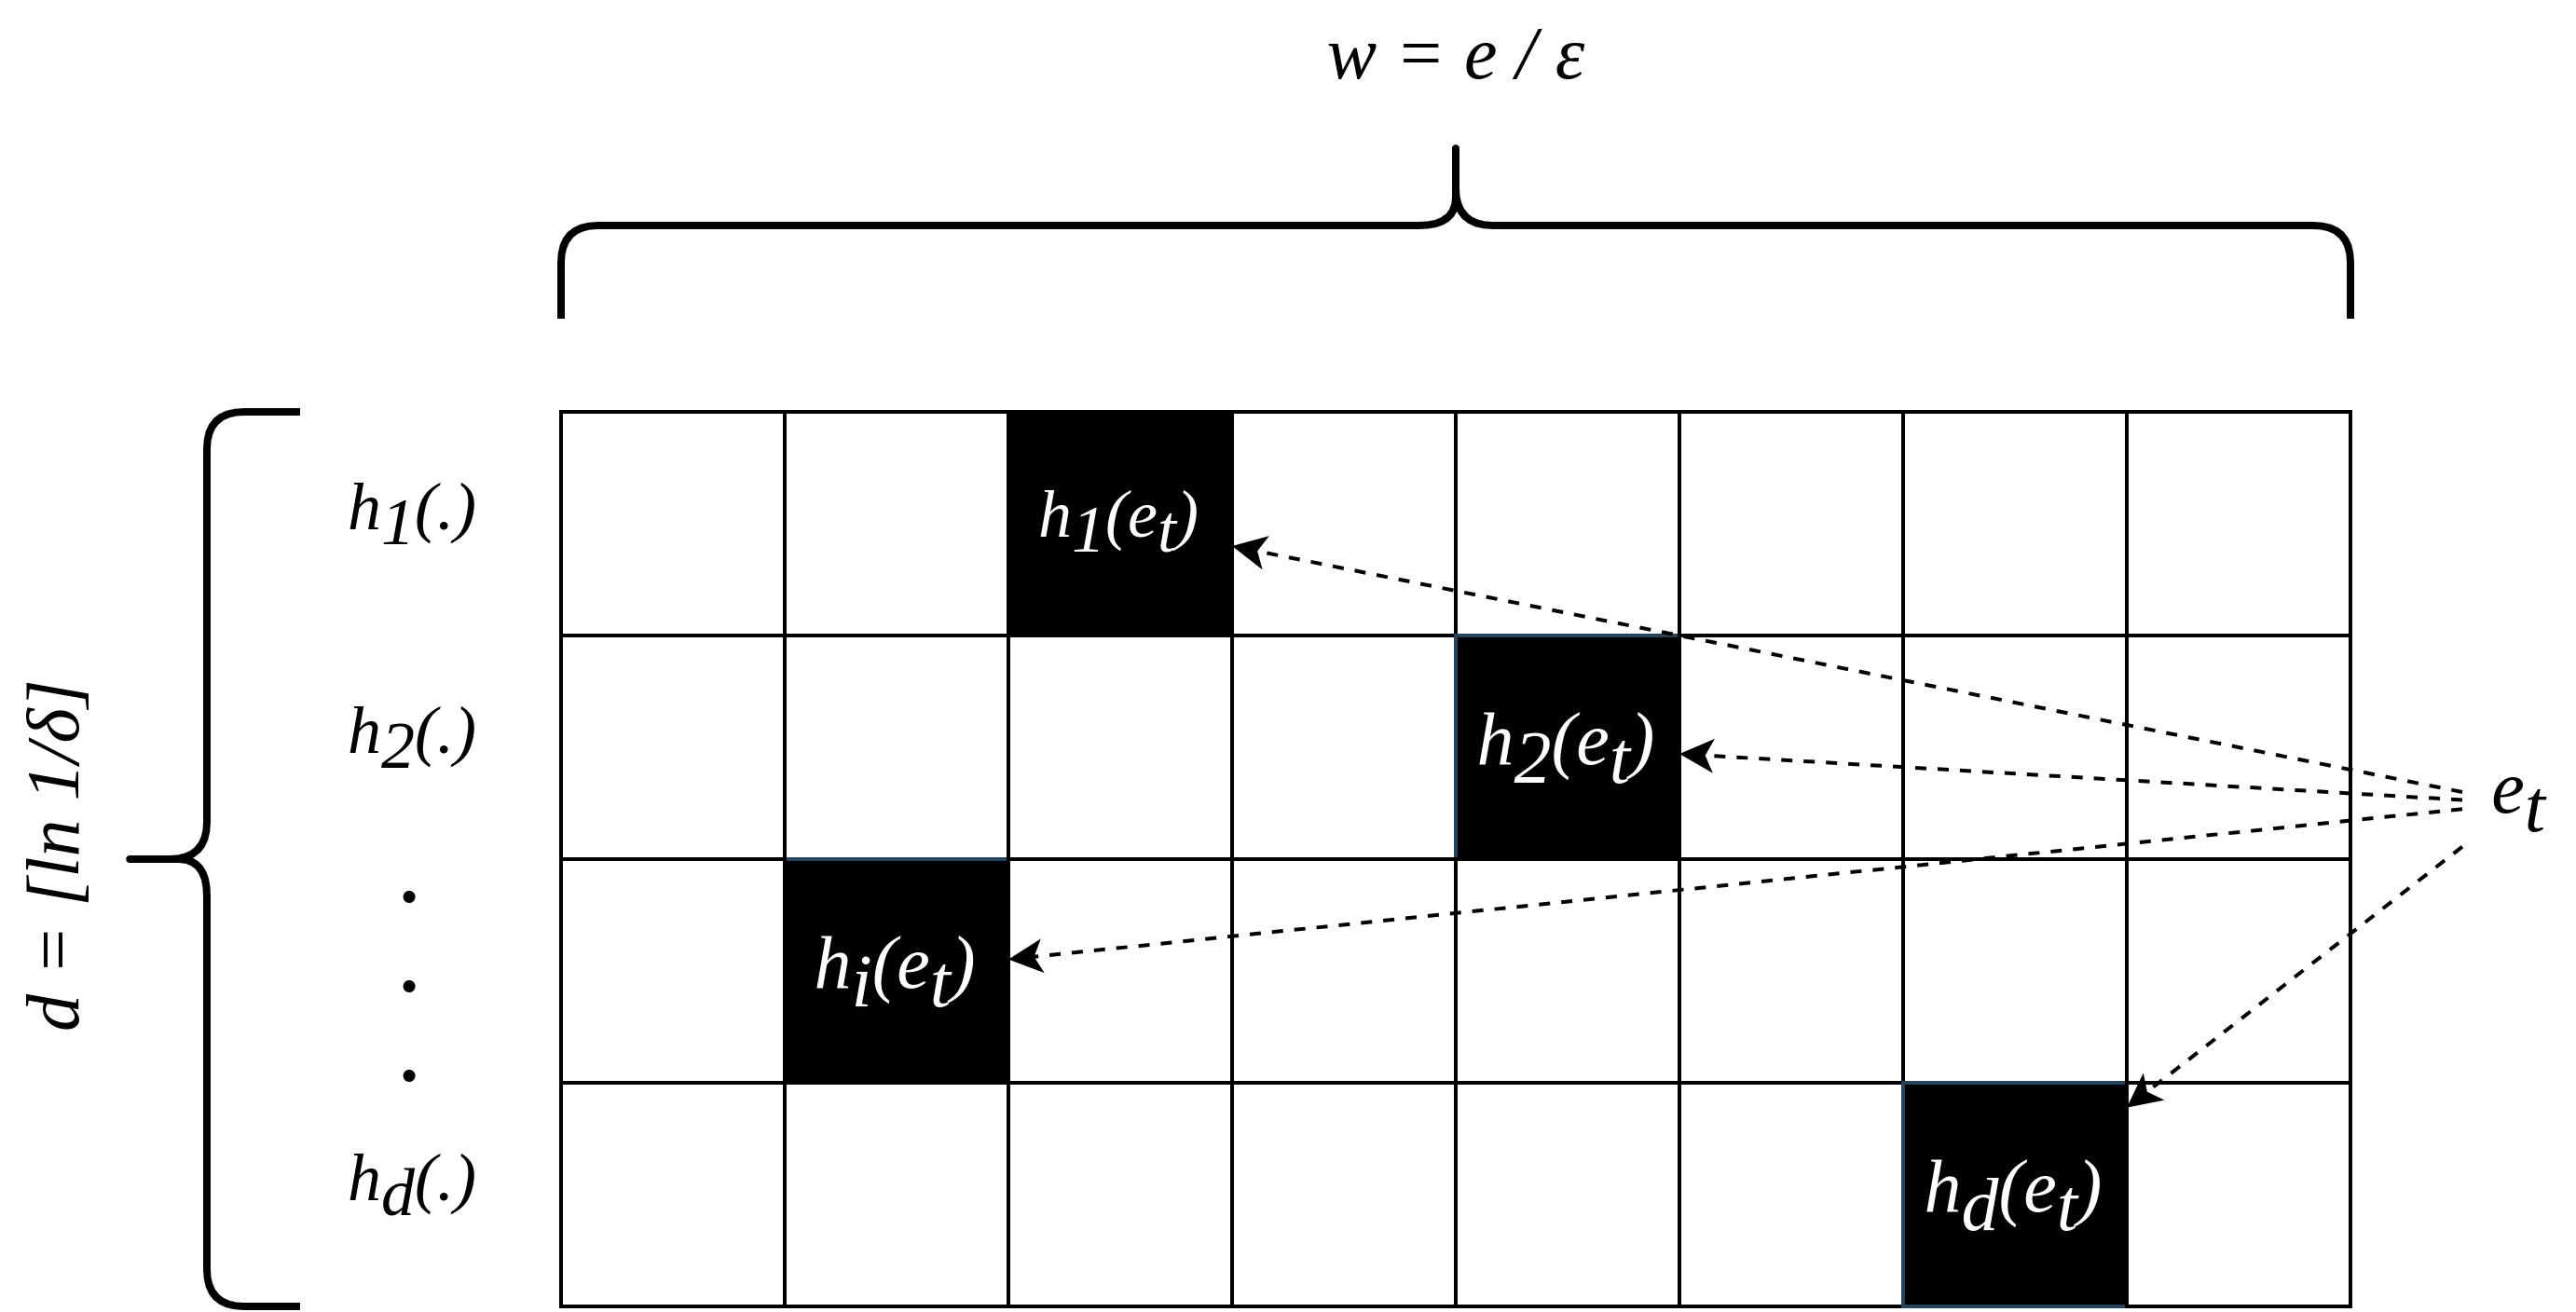
\includegraphics[width=0.5\textwidth]{img/countmin.png}}
    \caption{CountMin sketch\cite{zhao_gsketch:_2011}}
    \label{fig:countmin}
\end{figure}

\subsection{gSketch}

gSketch\cite{zhao_gsketch:_2011} is an extension of CountMin data structure. But unlike the CountMin sketch, this is specifically geared towards summarizing graph streams. gSketch is based on one of the below two assumptions.

\begin{itemize}
    \item A sample of the graph stream is available.
    \item Samples of both the graph stream and the query workload are available.
\end{itemize}

In CountMin, one global sketch is created for the entire stream. By doing so, it fails to take advantage of any structural properties present in the graph stream. gSketch tries to avoid this by considering the underlying structure of the graph stream using a sample. It then proceeds to partition its allocated space, as indicated in Fig.~\ref{fig:gsketch}. The goal of this partitioning step aims to maintain a sufficient frequency uniformity within each localized sketch in a way such that the combined error of the quarry estimations over the entire graph is kept at a minimum.

\begin{figure}[htbp]
    \centerline{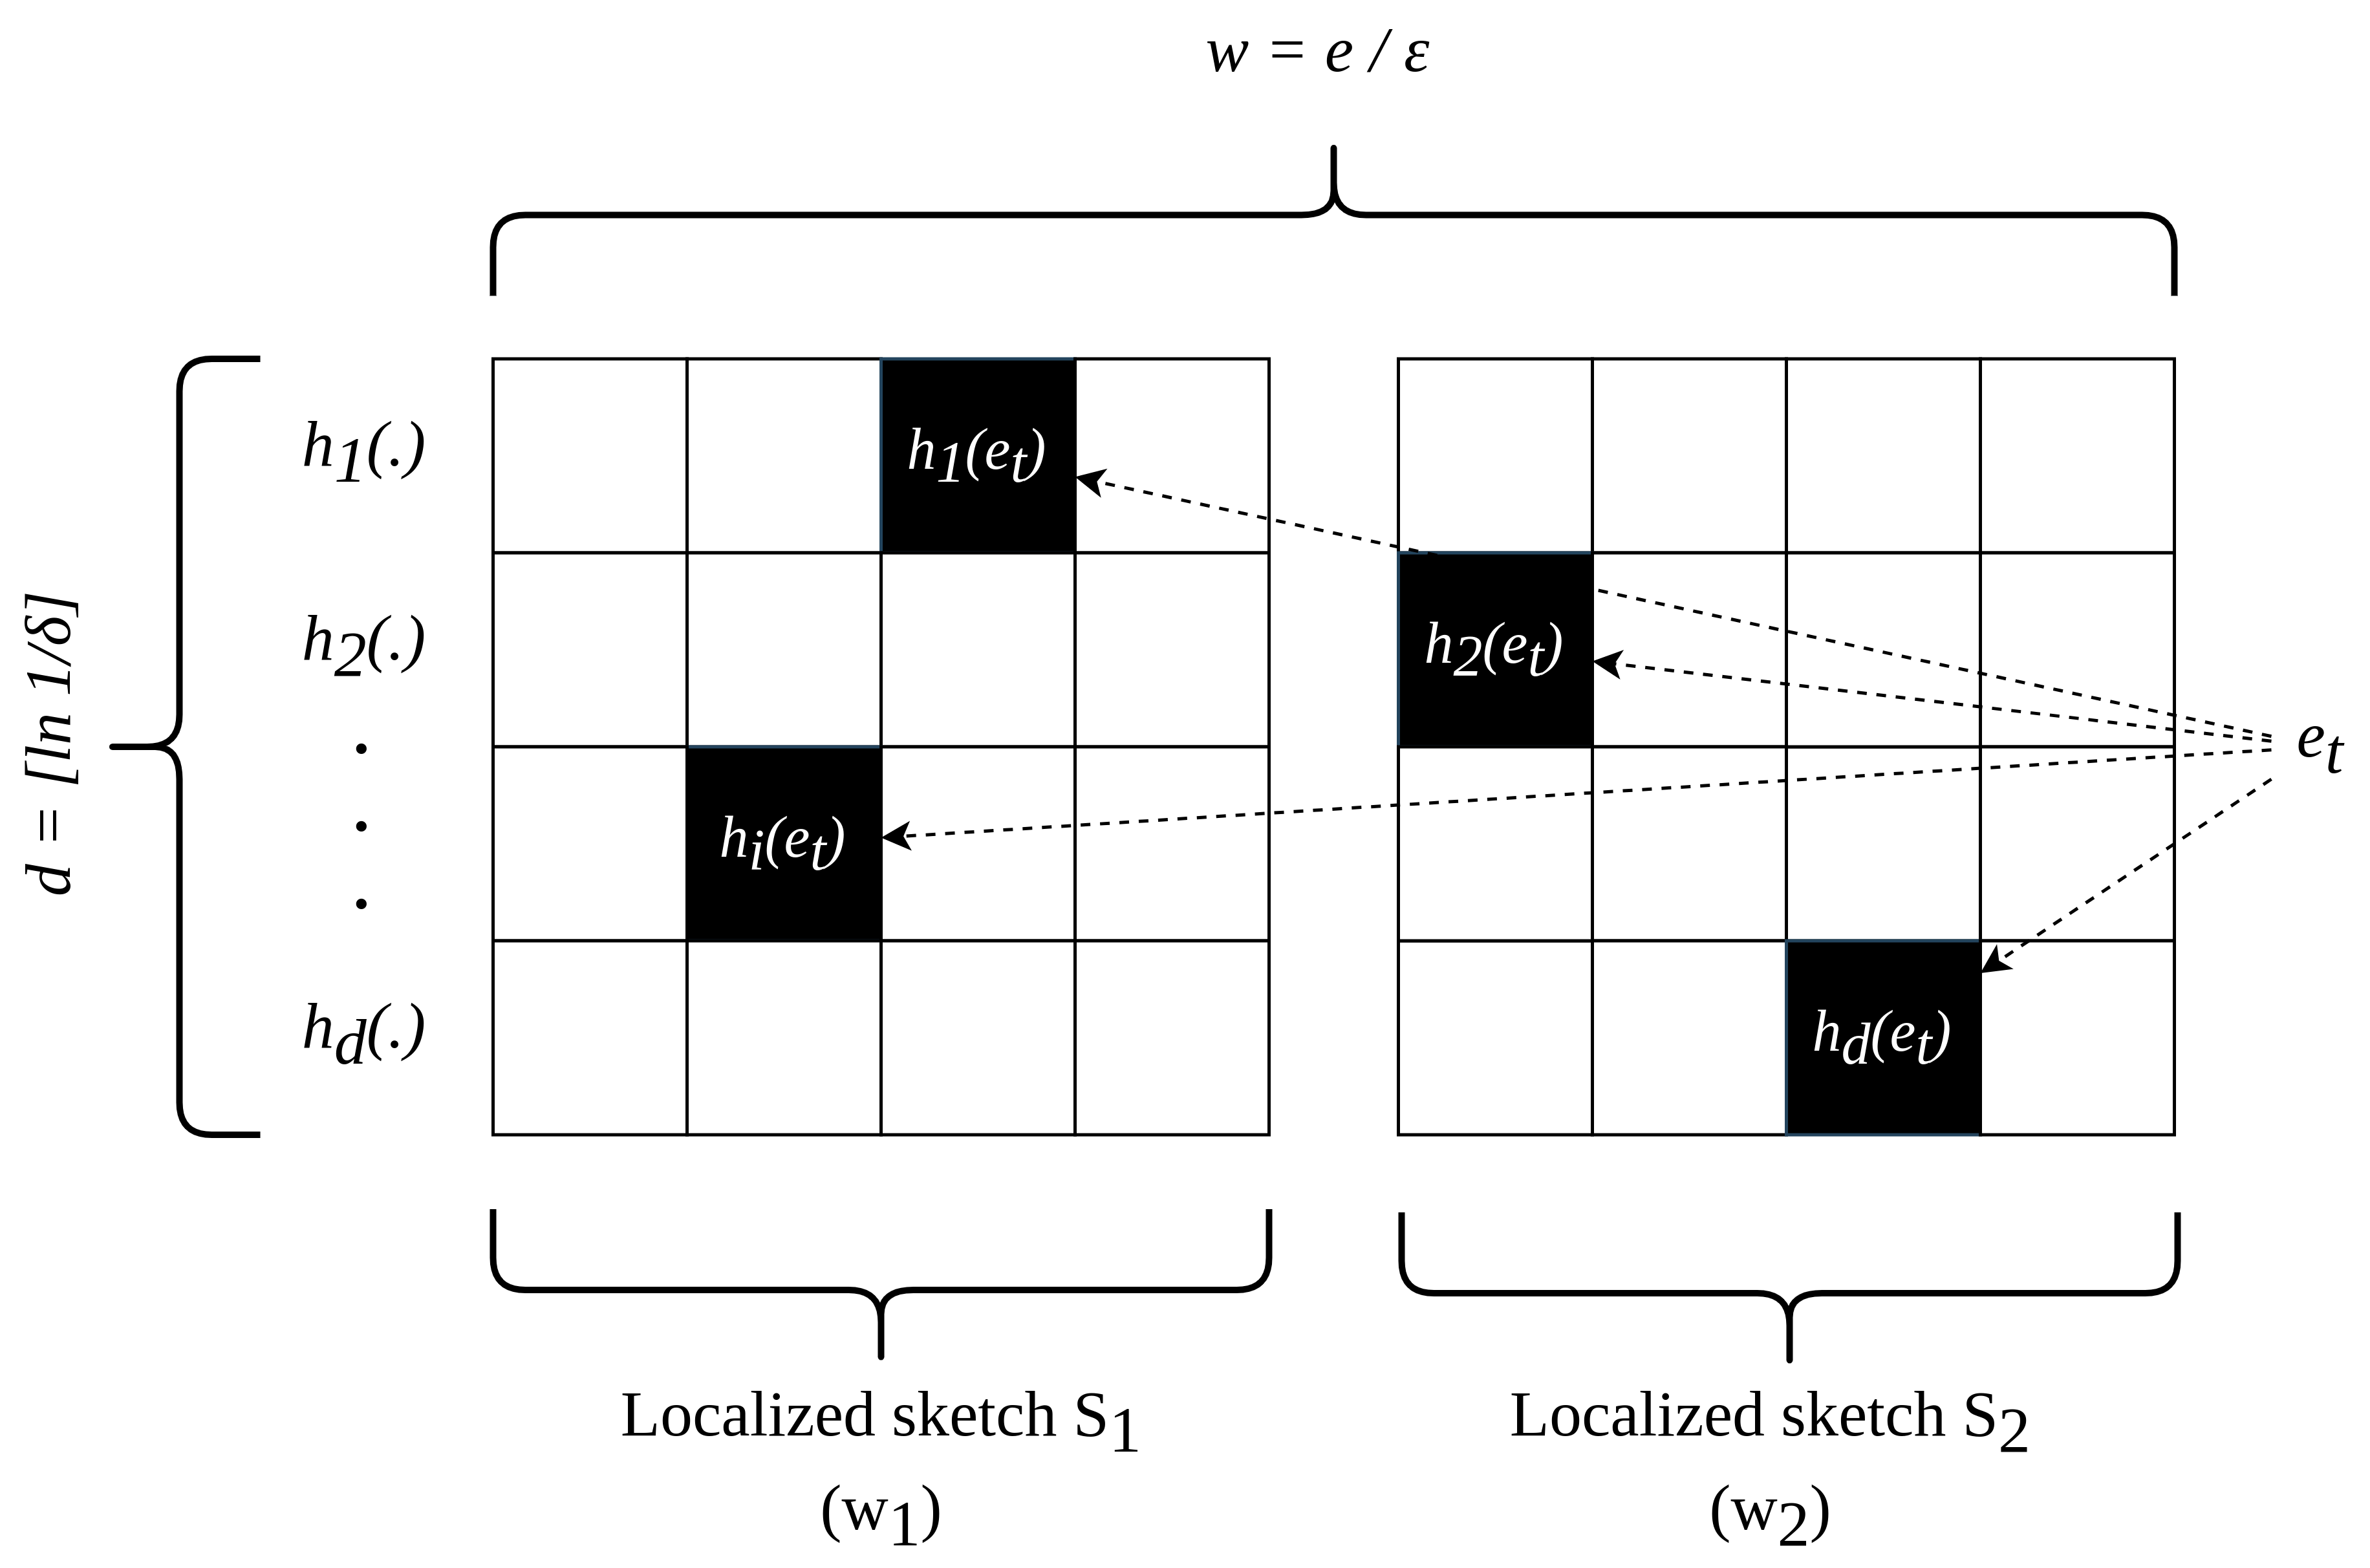
\includegraphics[width=0.5\textwidth]{img/gsketch.png}}
    \caption{gSketch sketch}
    \label{fig:gsketch}
\end{figure}

\subsection{TCM}

A disadvantage posed by all the approximate frequency count sketches like CountMin or gSketch is that they do not store the locality of the nodes. Therefore CountMin and gSketch cannot be used for conditional node queries or queries involving node connectivity. If these queries were to be run, the locality of the nodes has to be retained in the graph synopses. TCM\cite{tang_graph_2016} aims to solve this issue by storing the connectivity of the nodes in its data structure. TCM can summarize both node and edge information in constant time. Thus, it can answer a wide range of queries, unlike its predecessors. The structure of a TCM sketch is depicted in Fig.~\ref{fig:tcm}. TCM sketch could be considered as one of the pioneering works in summarizing data streams, which is directly related to our work presented in this paper.

\begin{figure}[htbp]
    \centerline{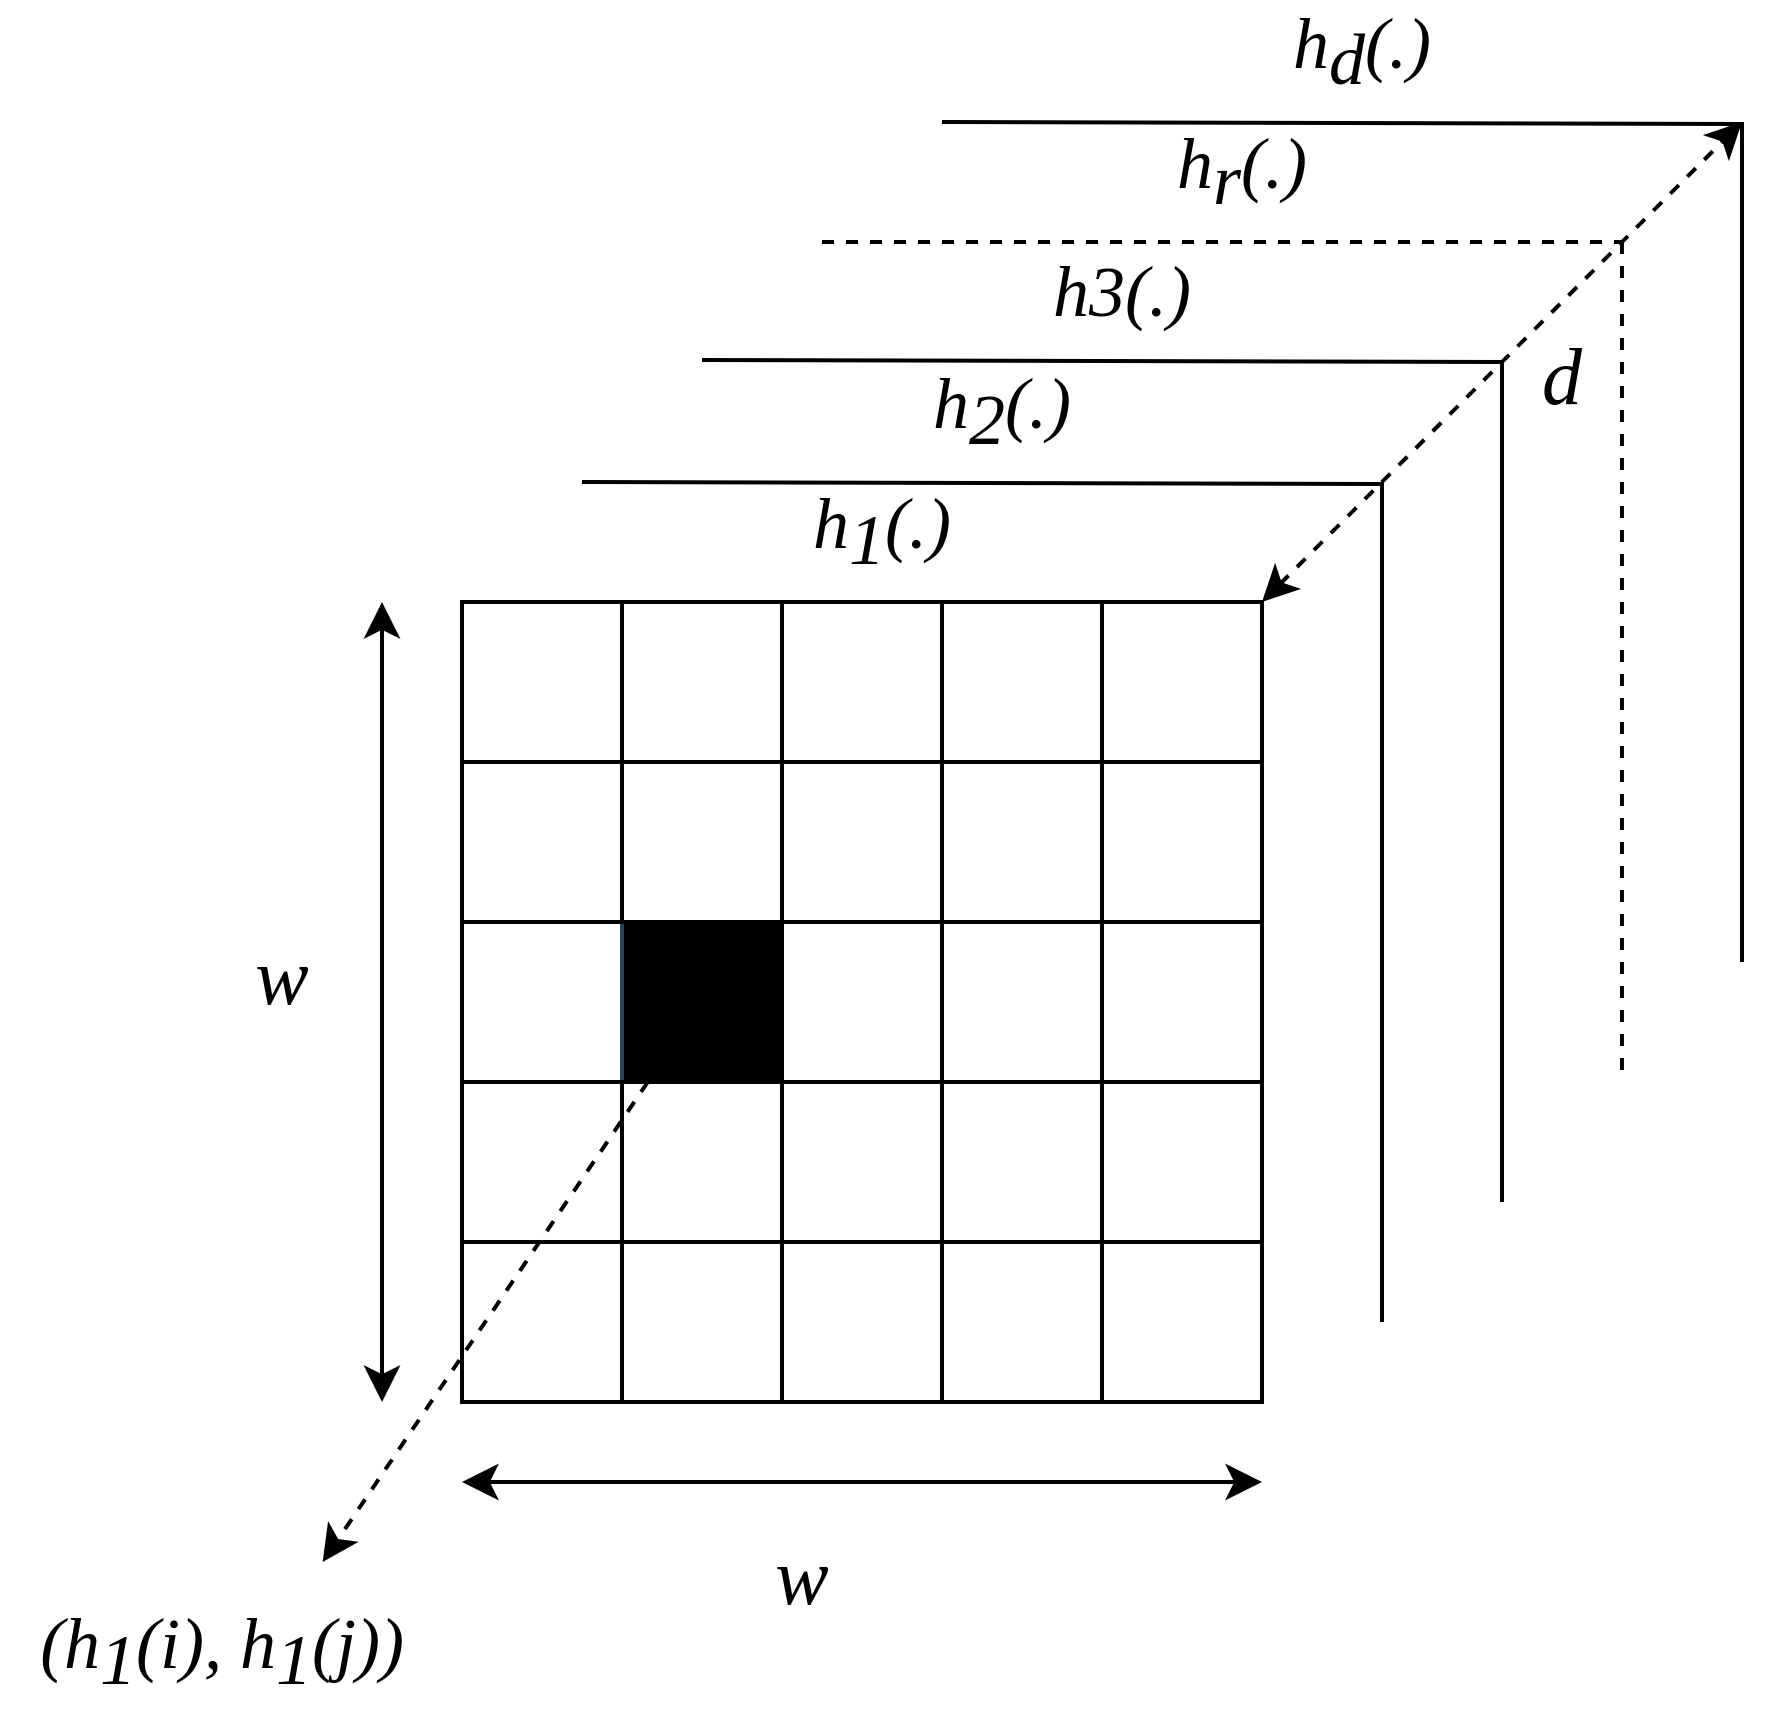
\includegraphics[width=0.35\textwidth]{img/tcm.png}}
    \caption{TCM sketch\cite{khan_query-friendly_2016}}
    \label{fig:tcm}
\end{figure}

\subsection{gMatrix}

The functionality of gMatrix\cite{khan_query-friendly_2016} is very similar to the TCM sketch. However, gMatrix considers several aspects which the TCM sketch does not address.

\begin{itemize}
    \item Reverse hashing queries through pairwise independent hash functions.
    \item Alternative options to extend sketch and space-saving synopses.
\end{itemize}

\section{Methodology}

\paragraph{}
The project will deal with large scale streaming and dynamic graphs. 
Therefore the first step would be obtaining available dataset of large 
natural graphs. One type of dataset that we will mainly focus on is the 
interactions of users in a social network. There are existing crawlers 
which are able to scrape things like tweets and facebook posts. We will also 
use a web crawler as suggested in the original work, to build a graph while 
the crawler is traversing through the web. “This is an unbounded graph since 
we do not know how large the graph would be and the graph keeps building while 
the crawler keeps traversing.”[11] And when it is within the acceptable 
boundary conditions of the research, we will use synthetic graphs to test 
out the algorithms and various corner cases. 

\paragraph{}
Then we will spend time on preparing an adequate environment for the sketching 
and partitioning operations to be run. There exists number of graph frameworks 
to facilitate graph computations such as Pregel, GraphLab, 
Distributed GraphLab, Giraph, Giraph++.  And data streaming frameworks 
like Apache Flink will be studied and used for the development purposes.  

\paragraph{}
Many streaming graph partitioning and sketching algorithms proposed by the 
previous researches haven’t made the codebase available along with the paper. 
So these will be re-implemented to be run on our environment of choice. In 
the researches where the sketching algorithms were proposed, there were 
evaluated against different types of queries, i.e edge queries, node queries 
and path queries. Reevaluating those with a similar set of parameters will 
help us in clearly differentiating the strengths and weaknesses of each 
sketching method. 

\paragraph{}
Hereafter, the implemented sketching mechanisms will be tested in evaluating 
other graph properties like KNN and K-furthest neighbor. There are various 
evaluating techniques proposed by the previous researches in evaluating the 
sketching mechanisms such as Average Relative Error and Number of Effective 
Queries\cite{kumarage_efficient_2017}. And other resource factors such as memory 
usage will also be measured in each test. 

\paragraph{}
After proper evaluation of the strengths and weaknesses of existing methods 
with respect to different graph properties, we will research on improving those 
methods. And we will attempt at proposing how which technique performs better 
when evaluating each graph property. 

\paragraph{}
In the final phase of the project, we will focus on evaluating the models on 
top of a parallel framework as the future work of the original research 
suggests\cite{kumarage_efficient_2017}. And then we will re-evaluate the proposed 
improvements on top of the parallel framework to report any performance 
gained in running them parallelly. 

\section{Implementation}
\label{sec:implementation}

\subsection{Experimental Setup}

The implementation mainly consists of two components; the test suite and the sketching algorithms. The entire code-base has been written in Python 3.8. All the tests were run on a 12-core Ryzen 3900 machine with a base clock of 3.1GHz and 32 GB RAM. However, only one core was utilized in running the tests. 

% The architecture of the benchmarking test suit is shown in Fig.~\ref{fig:test_suite}. It was designed in a modular way such that it permits easy addition of more test cases and graph sketches when necessary. 

% \begin{figure}[htbp]
%     \centerline{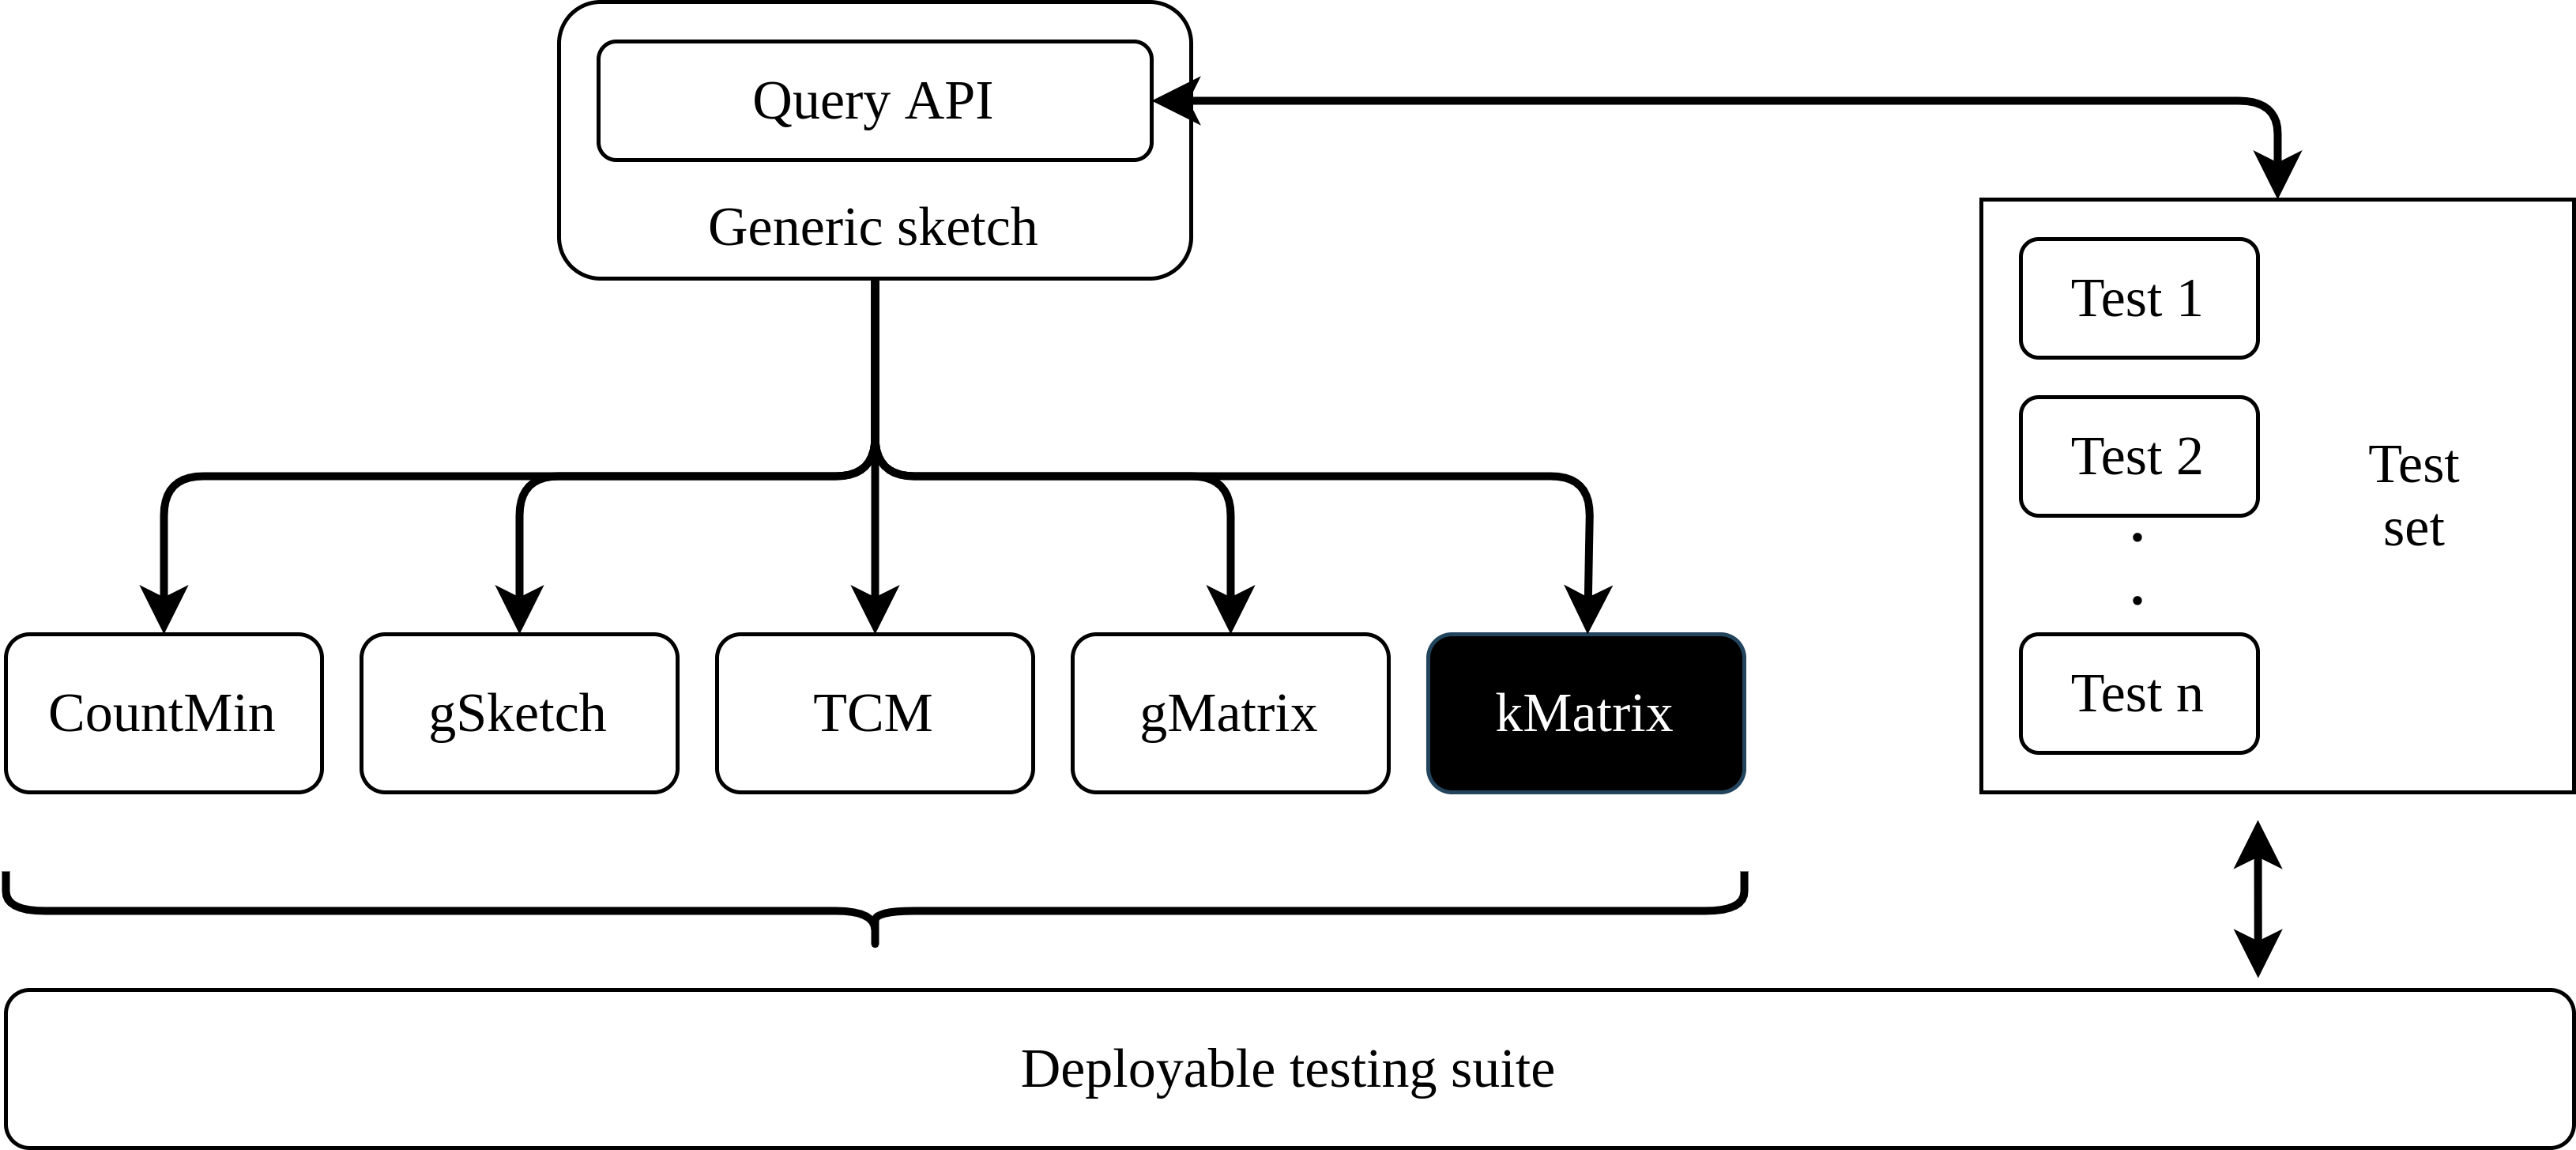
\includegraphics[width=0.5\textwidth]{img/test_suite.png}}
%     \caption{High level architecture of the test suite}
%     \label{fig:test_suite}
% \end{figure}

A sample of 30,000 edges has been extracted from relevant datasets for initializing kMatrix at the beginning of each experiment. This sample stream has been obtained using reservoir sampling. 

\subsection{Datasets}

3 datasets were chosen to carry out the benchmarking process in this research. These were chosen to represent different application domains. 

\paragraph{unicorn-wget\cite{DVN/5H4TDI_2018}}
unicorn-wget is a dataset created from capturing the packet information of the network activity of a simulated network. This dataset was created at Harvard University. The dataset consists of 5 parts. From them, Hour-Long Wget Benign Dataset (Base Graph) which consist of 17,778 nodes and 2,779,726 edges was chosen for the experiment. We filtered 10\% of the edges using reservoir sampling for our experiments. 

\paragraph{email-EuAll\cite{leskovec_graph_2007}}
This data was extracted using email data from a large European research institution. The dataset consists of emails sent out in a period of 18 months. Each data item contains sender, receiver and the time of the origination of each email. The dataset consisted of 265,214 nodes and 420,045 edges\cite{noauthor_snap_nodate_email}. 

% \paragraph{cit-HepPh\cite{leskovec_graphs_2005, gehrke_overview_2003}}
\paragraph{cit-HepPh\cite{gehrke_overview_2003}}
cit-HepPh citation graph is from the e-print arXiv regarding high energy physics phenomenology. It has 34,546 papers (nodes) and 421,578 citations (edges). We used the full dataset in our experiments. 

\subsection{Evaluation Metrics}
\label{section:design_evaluation_metrics}

\subsubsection{Average Relative Error (ARE)}
\label{section:metrics_are}

The relative error \(er(Q)\) of a query \(Q\) is defined as \eqref{eq:9} where \(\tilde{f}'(Q)\) and \(f(Q)\) is the estimated frequency and the true frequency of the query respectively.

\begin{equation}
    er(Q) =  \frac{\tilde{f}'(Q) - f(Q)}{f(Q)} = \frac{\tilde{f}'(Q)}{f(Q)} -1
    \label{eq:9}
\end{equation}

Given a set of m queries, $\{ Q_1 , ....., Q_m \}$, the average relative error is defined by taking the average of the relative error of all queries $Q_i$ for \(i \in [1,m]\).

\begin{equation}
    e(Q) =  \frac{\sum_{i=1}^{k} er(Q_i)}{m}
\end{equation}

\subsubsection{Number of Effective Queries (NEQ)}
\label{section:metrics_neq}

A query is said to be effective if the error, $\tilde{f}'(Q) - f(Q), \leq G_0$,  where $G_0$ is a predefined value. The number of effective queries is defined as,

\begin{equation}
    g(Q) =  |\{\,q\, | \, (\tilde{f}'(q) - f(q)) \leq G_0, \,q\, \epsilon \,Q\}|
\end{equation}

% This can also be expressed as a percentage of effective queries (PEQ).

% \begin{equation}
%     g(Q) =  \frac{\left | \{\,q\, |   \left |\tilde{f}'(q) - f(q)\right | \leq G_0, \,q \, \epsilon  \,Q\} \, \right|}{|Q|}*100
% \end{equation}

\section{Results}
\label{sec:results}

This section will describe all the experiments conducted to measure the effectiveness of kMatrix against existing streaming graph sketching techniques. 

We have considered CountMin, gSketch, TCM, gMatrix and kMatrix sketches in our experiments. These sketches can be categorized into two groups depending on the type of queries they are able to answer.

\begin{enumerate}
    \item \emph{Type I} - The sketches which support only the edge frequency queries, i.e. CountMin and gSketch.
    \item \emph{Type II} - The sketches which support many graph queries in general, i.e. TCM, gMatrix and kMatrix
\end{enumerate}

Since \emph{Type I} sketches cannot answer anything other than edge frequency queries, we have only included \emph{Type II} sketches in our comparisons against kMatrix.

\subsection{Build-time}

Here we investigated the time to add the entire dataset to the sketch. The sketches were allocated a constant memory size of 1 MB, and the number of hash functions was set to \(d = 7\). The edges were streamed at the maximum throughput of each sketch. Therefore this experiment gives an idea about the average insertion rate of edges for each sketch. A minor drawback of kMatrix is that it takes some time for its initialization stage. However, this initialization time becomes negligible compared to the advantage that kMatrix receives over time due to its faster streaming rate. In both Fig.~\ref{fig:btt-a} and Fig.~\ref{fig:btt-c}, it has managed to outperform other sketching techniques by a significant margin. In Fig.~\ref{fig:btt-b}, kMatrix has shown comparable performance to gMatrix. With the increase of the data contained within the sketch, the number of hash collisions in TCM and gMatrix has grown over time, increasing the computational cost of inserting a new edge. kMatrix has maintained a relatively lower build time as a result of its lower number of hash collisions due to the sketch partitioning before inserting the edges.

\begin{figure}[htbp] 
    \centering
    \subfloat[unicorn-wget\label{fig:btt-a}]{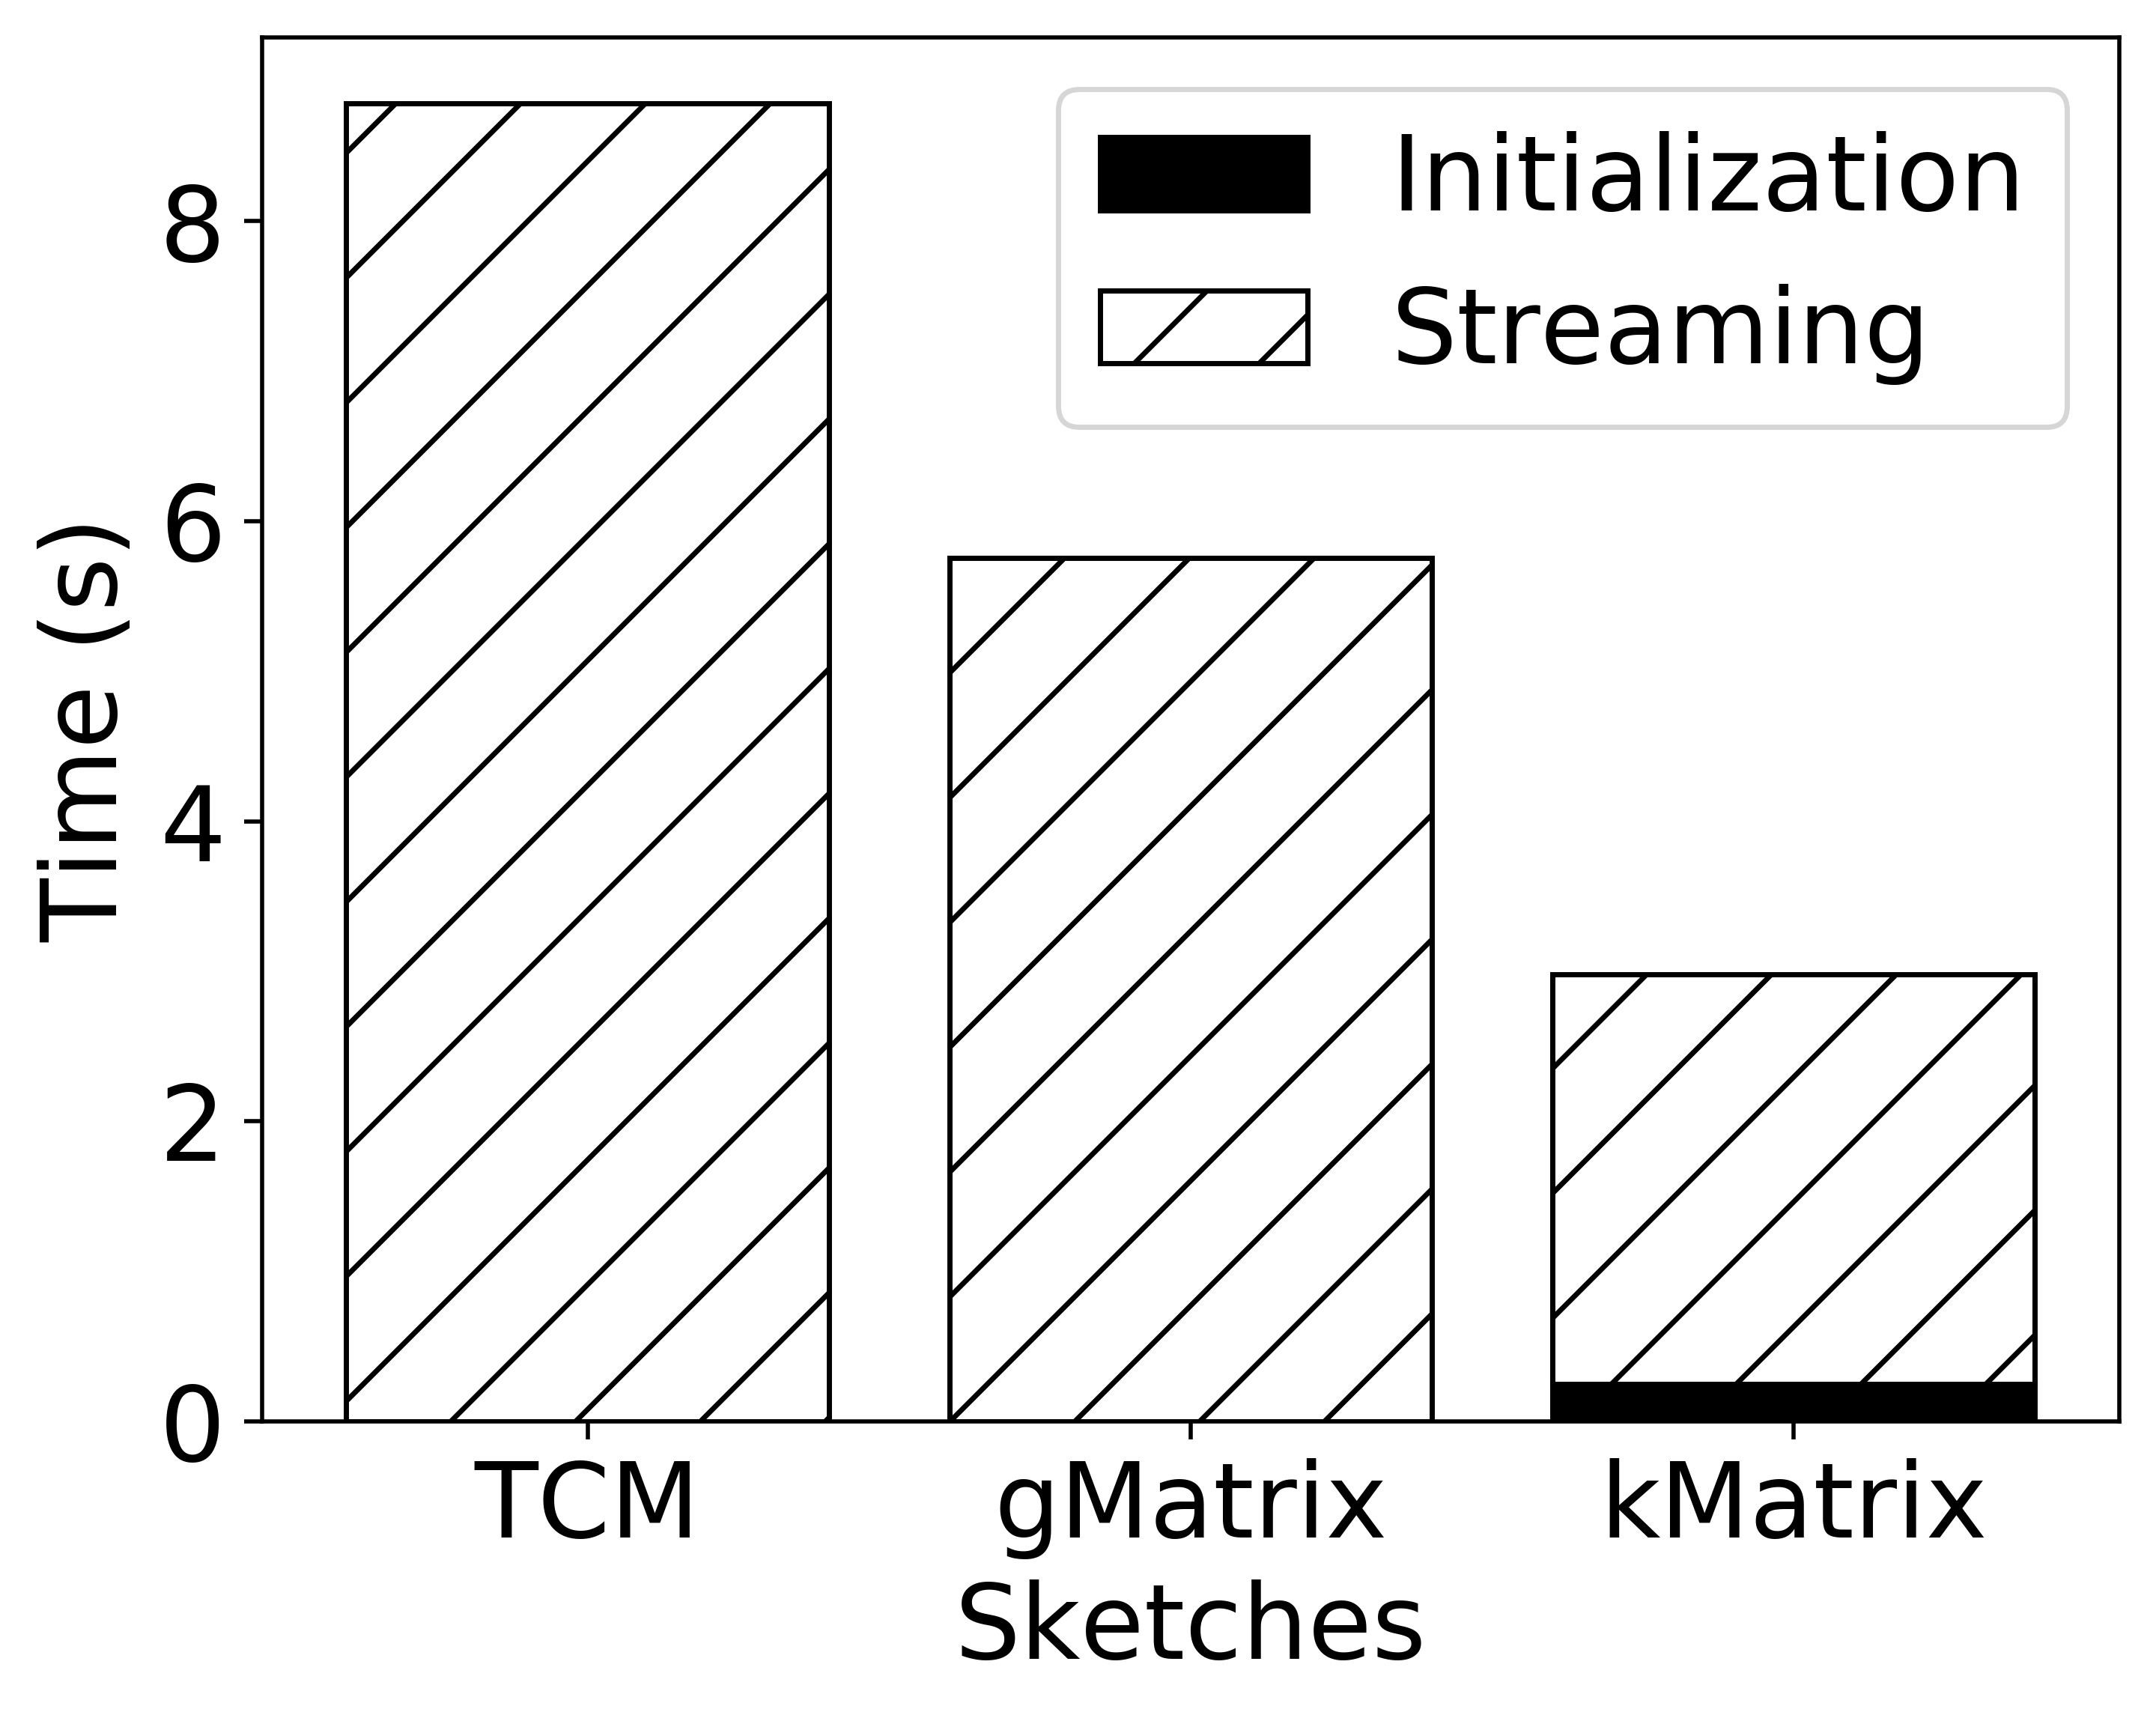
\includegraphics[width=0.45\linewidth]{img/buildtime_1024_unicorn-wget.png}}
    \hfill
    \subfloat[email-EuAll\label{fig:btt-b}]{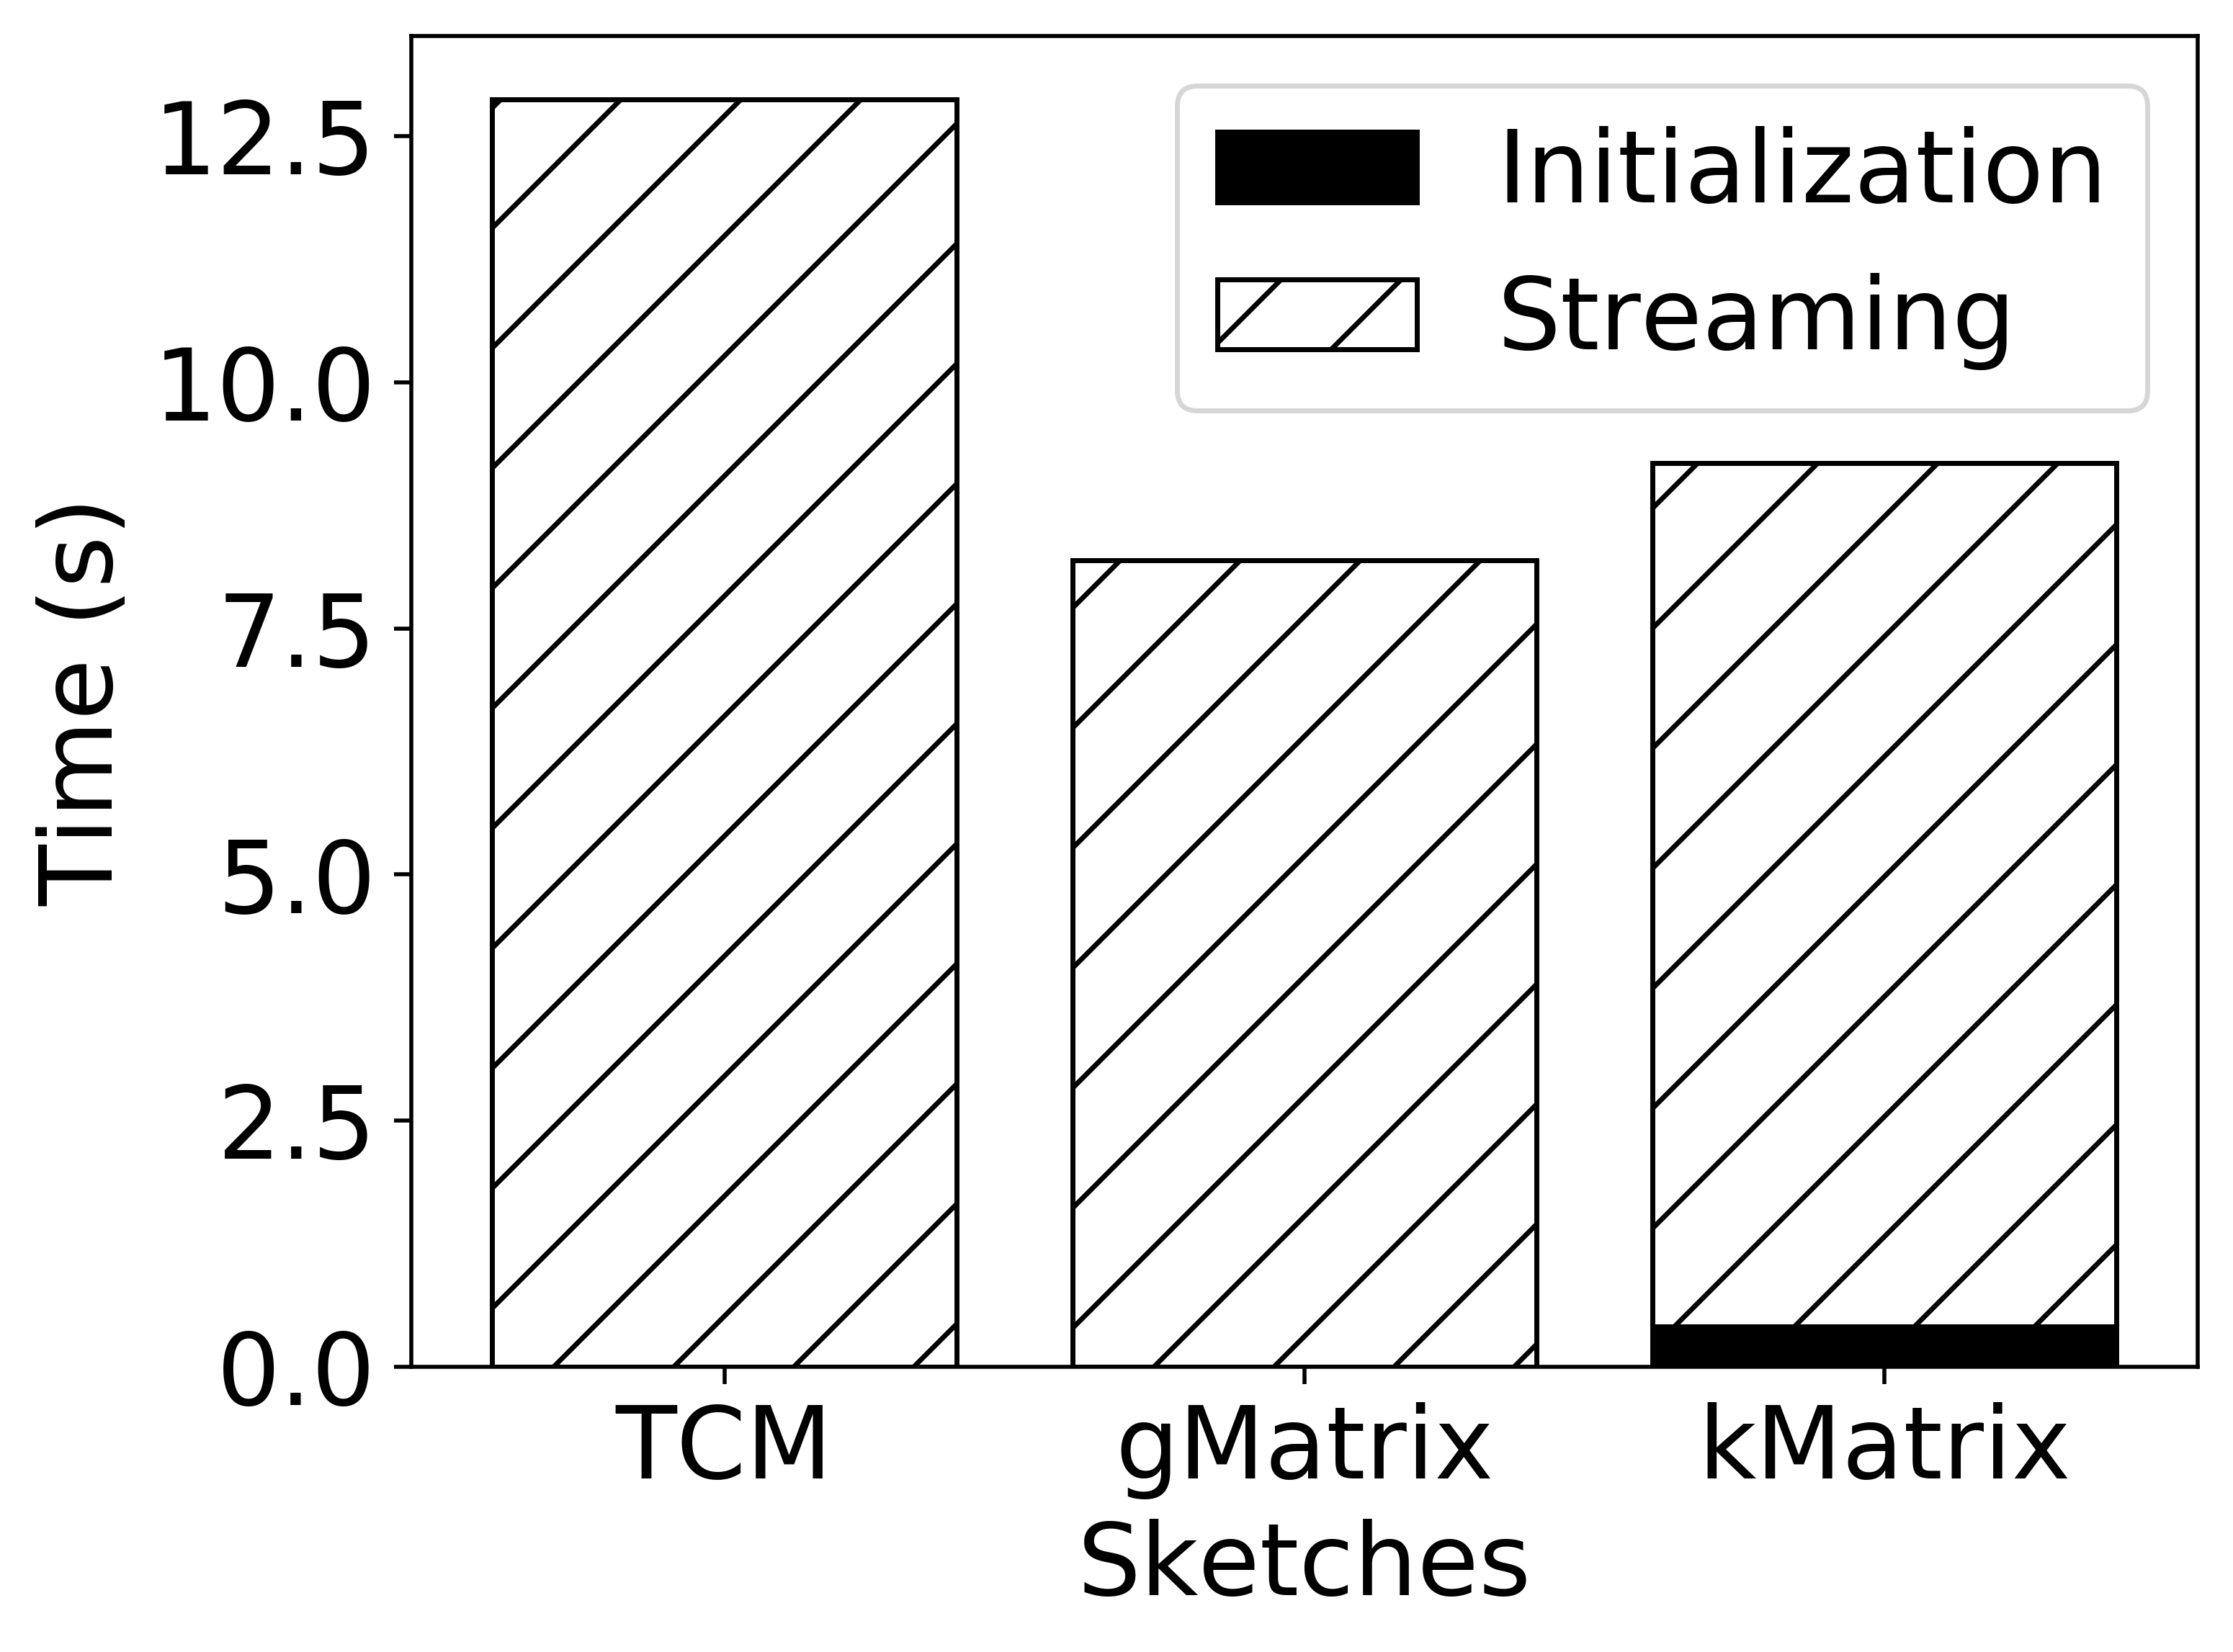
\includegraphics[width=0.45\linewidth]{img/buildtime_1024_email-EuAll.png}}
    \hfill
    \subfloat[cit-HepPh\label{fig:btt-c}]{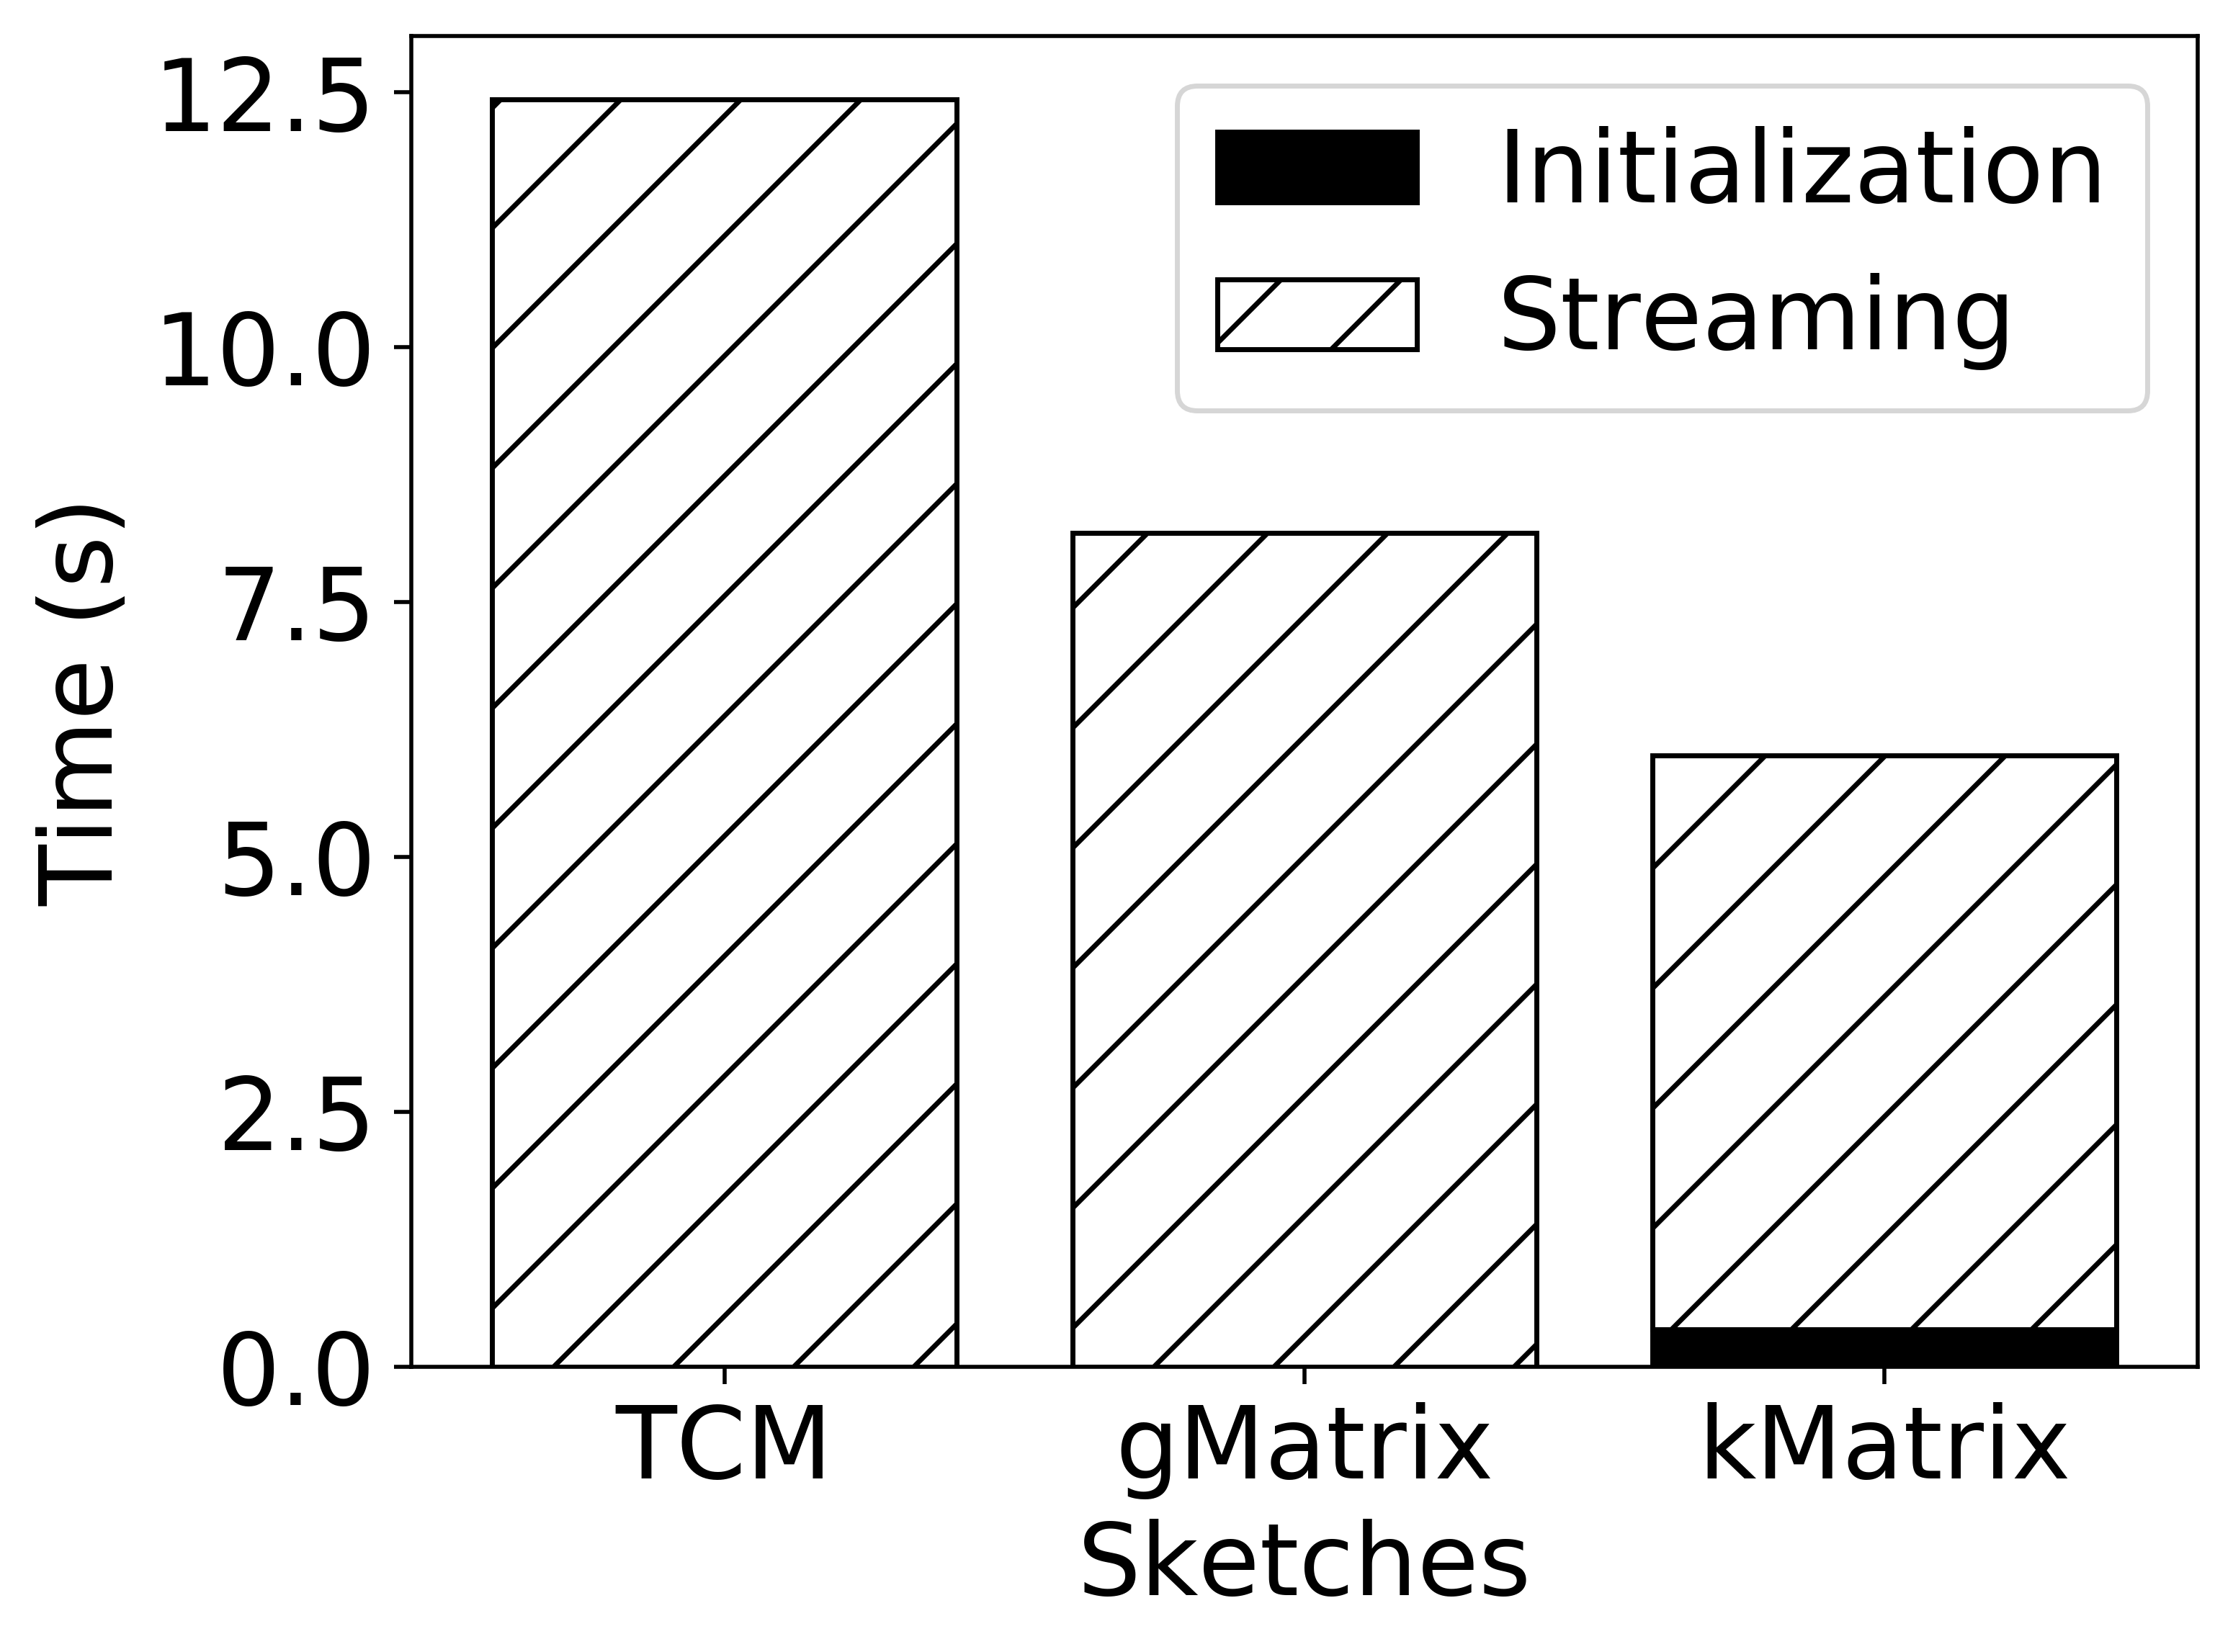
\includegraphics[width=0.45\linewidth]{img/buildtime_1024_cit-HepPh.png}}
    \caption{Build-time}
    \label{fig:buildtime-test}
\end{figure}

\subsection{Edge queries}

This experiment investigates how accurately the kMatrix can answer the edge queries after the summarization process. For this, we let our datastream get summarized into the sketch and then queried the frequency of different edges chosen at random. The experiment was repeated for each sketch for the sizes, 200 KB, 300 KB, 400 KB and 512 KB while keeping the number of hash functions at \(d = 7\). We have used average relative error and the number of effective queries as the evaluation matrices for this experiment.

\subsubsection{Average Relative Error}
\label{section:results_are}

\begin{figure}[htbp] 
    \centering
    \subfloat[unicorn-wget\label{fig:are-a}]{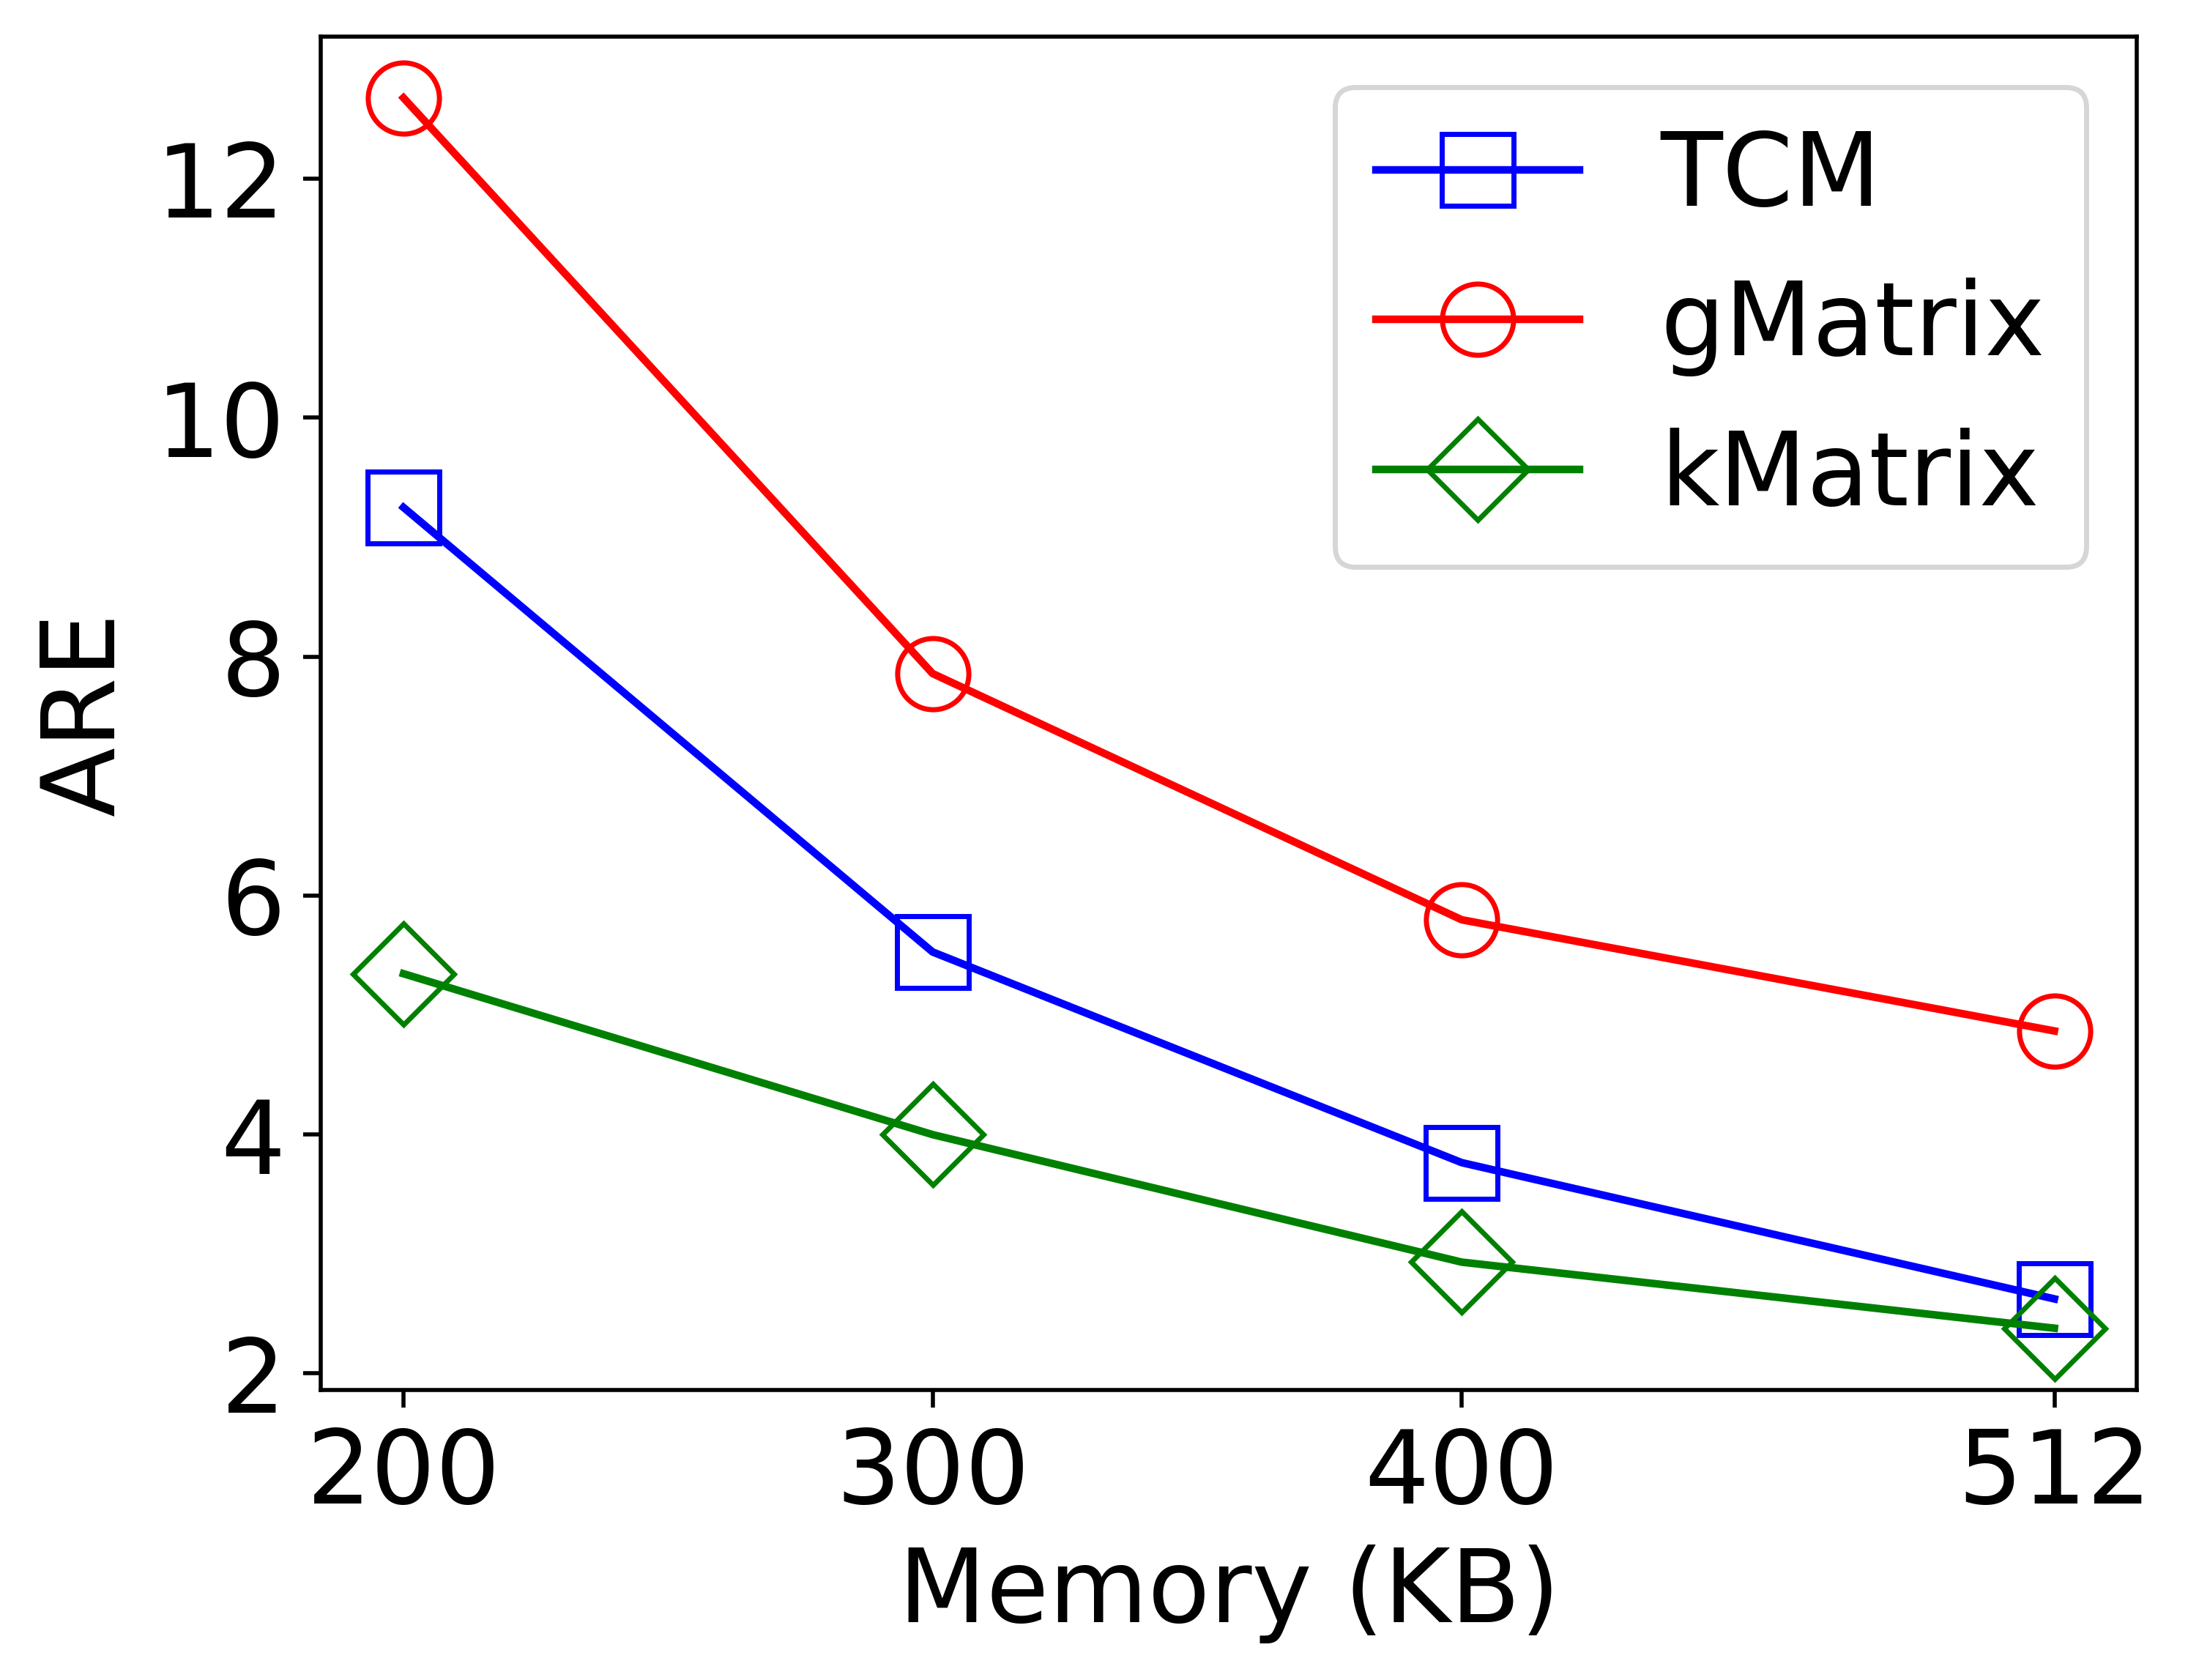
\includegraphics[width=0.45\linewidth]{img/edge_query_are_unicorn-wget.png}}
    \hfill
    \subfloat[email-EuAll\label{fig:are-b}]{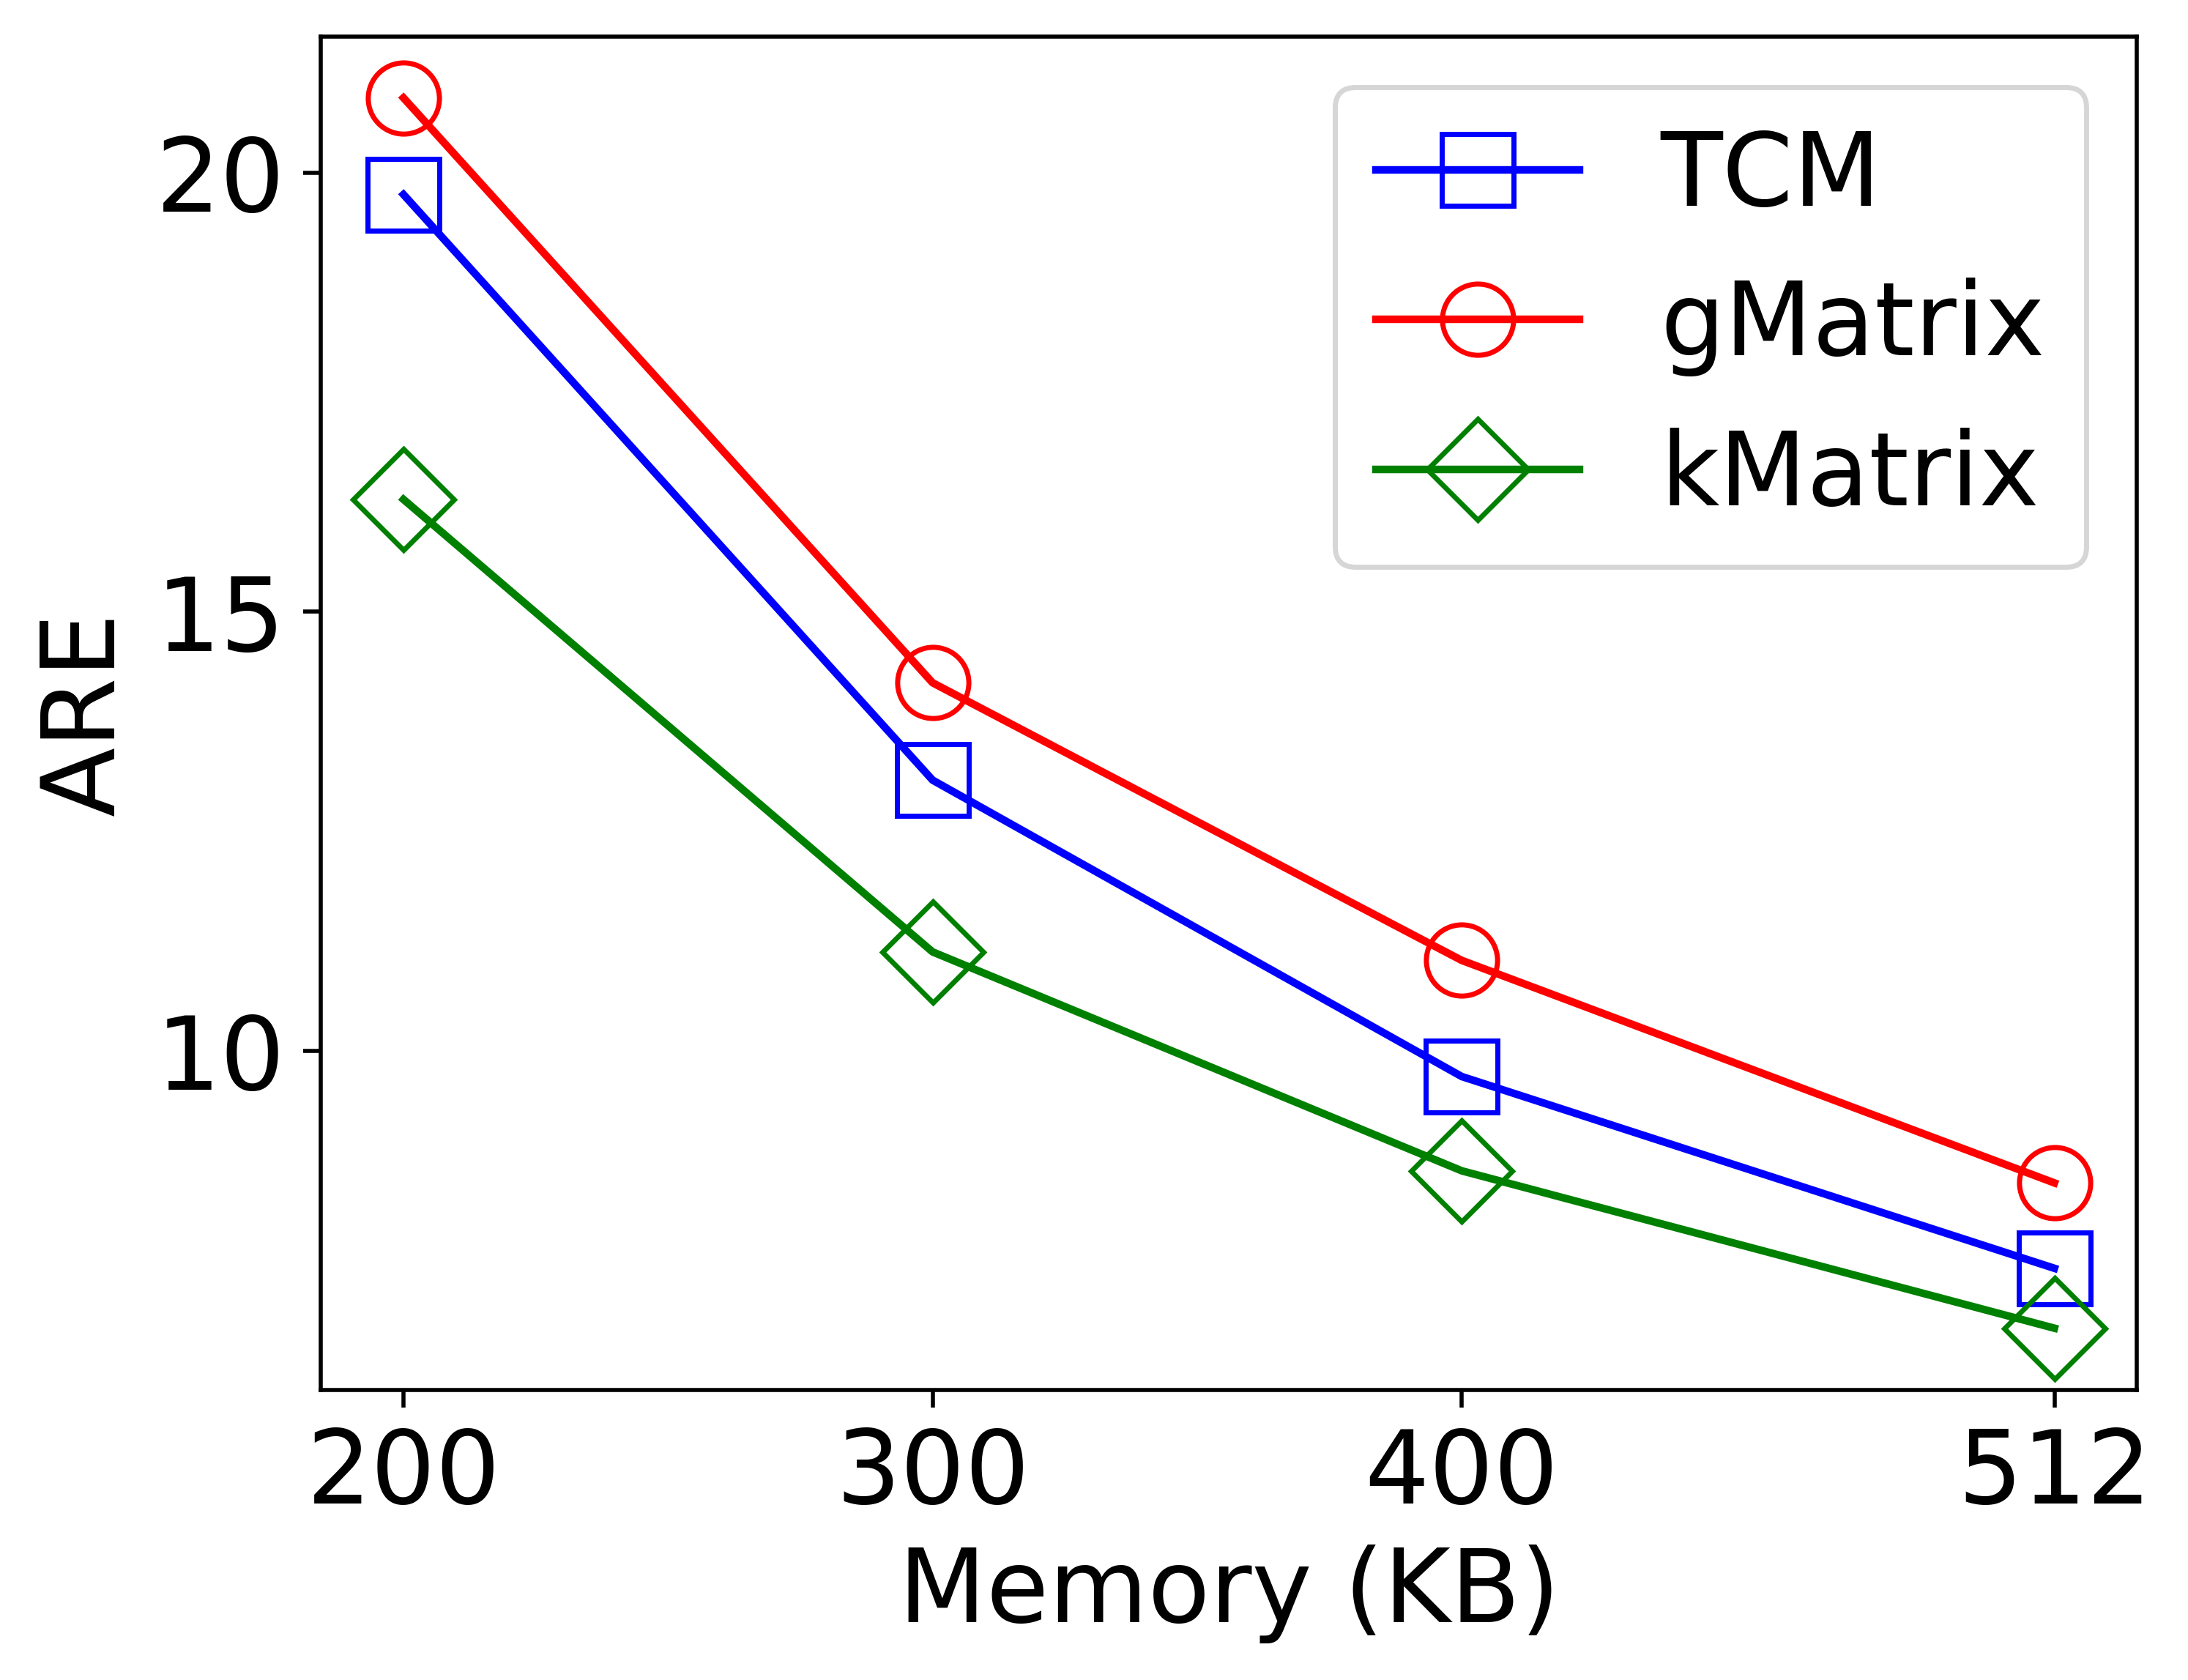
\includegraphics[width=0.45\linewidth]{img/edge_query_are_email-EuAll.png}}
    \hfill
    \subfloat[cit-HepPh\label{fig:are-c}]{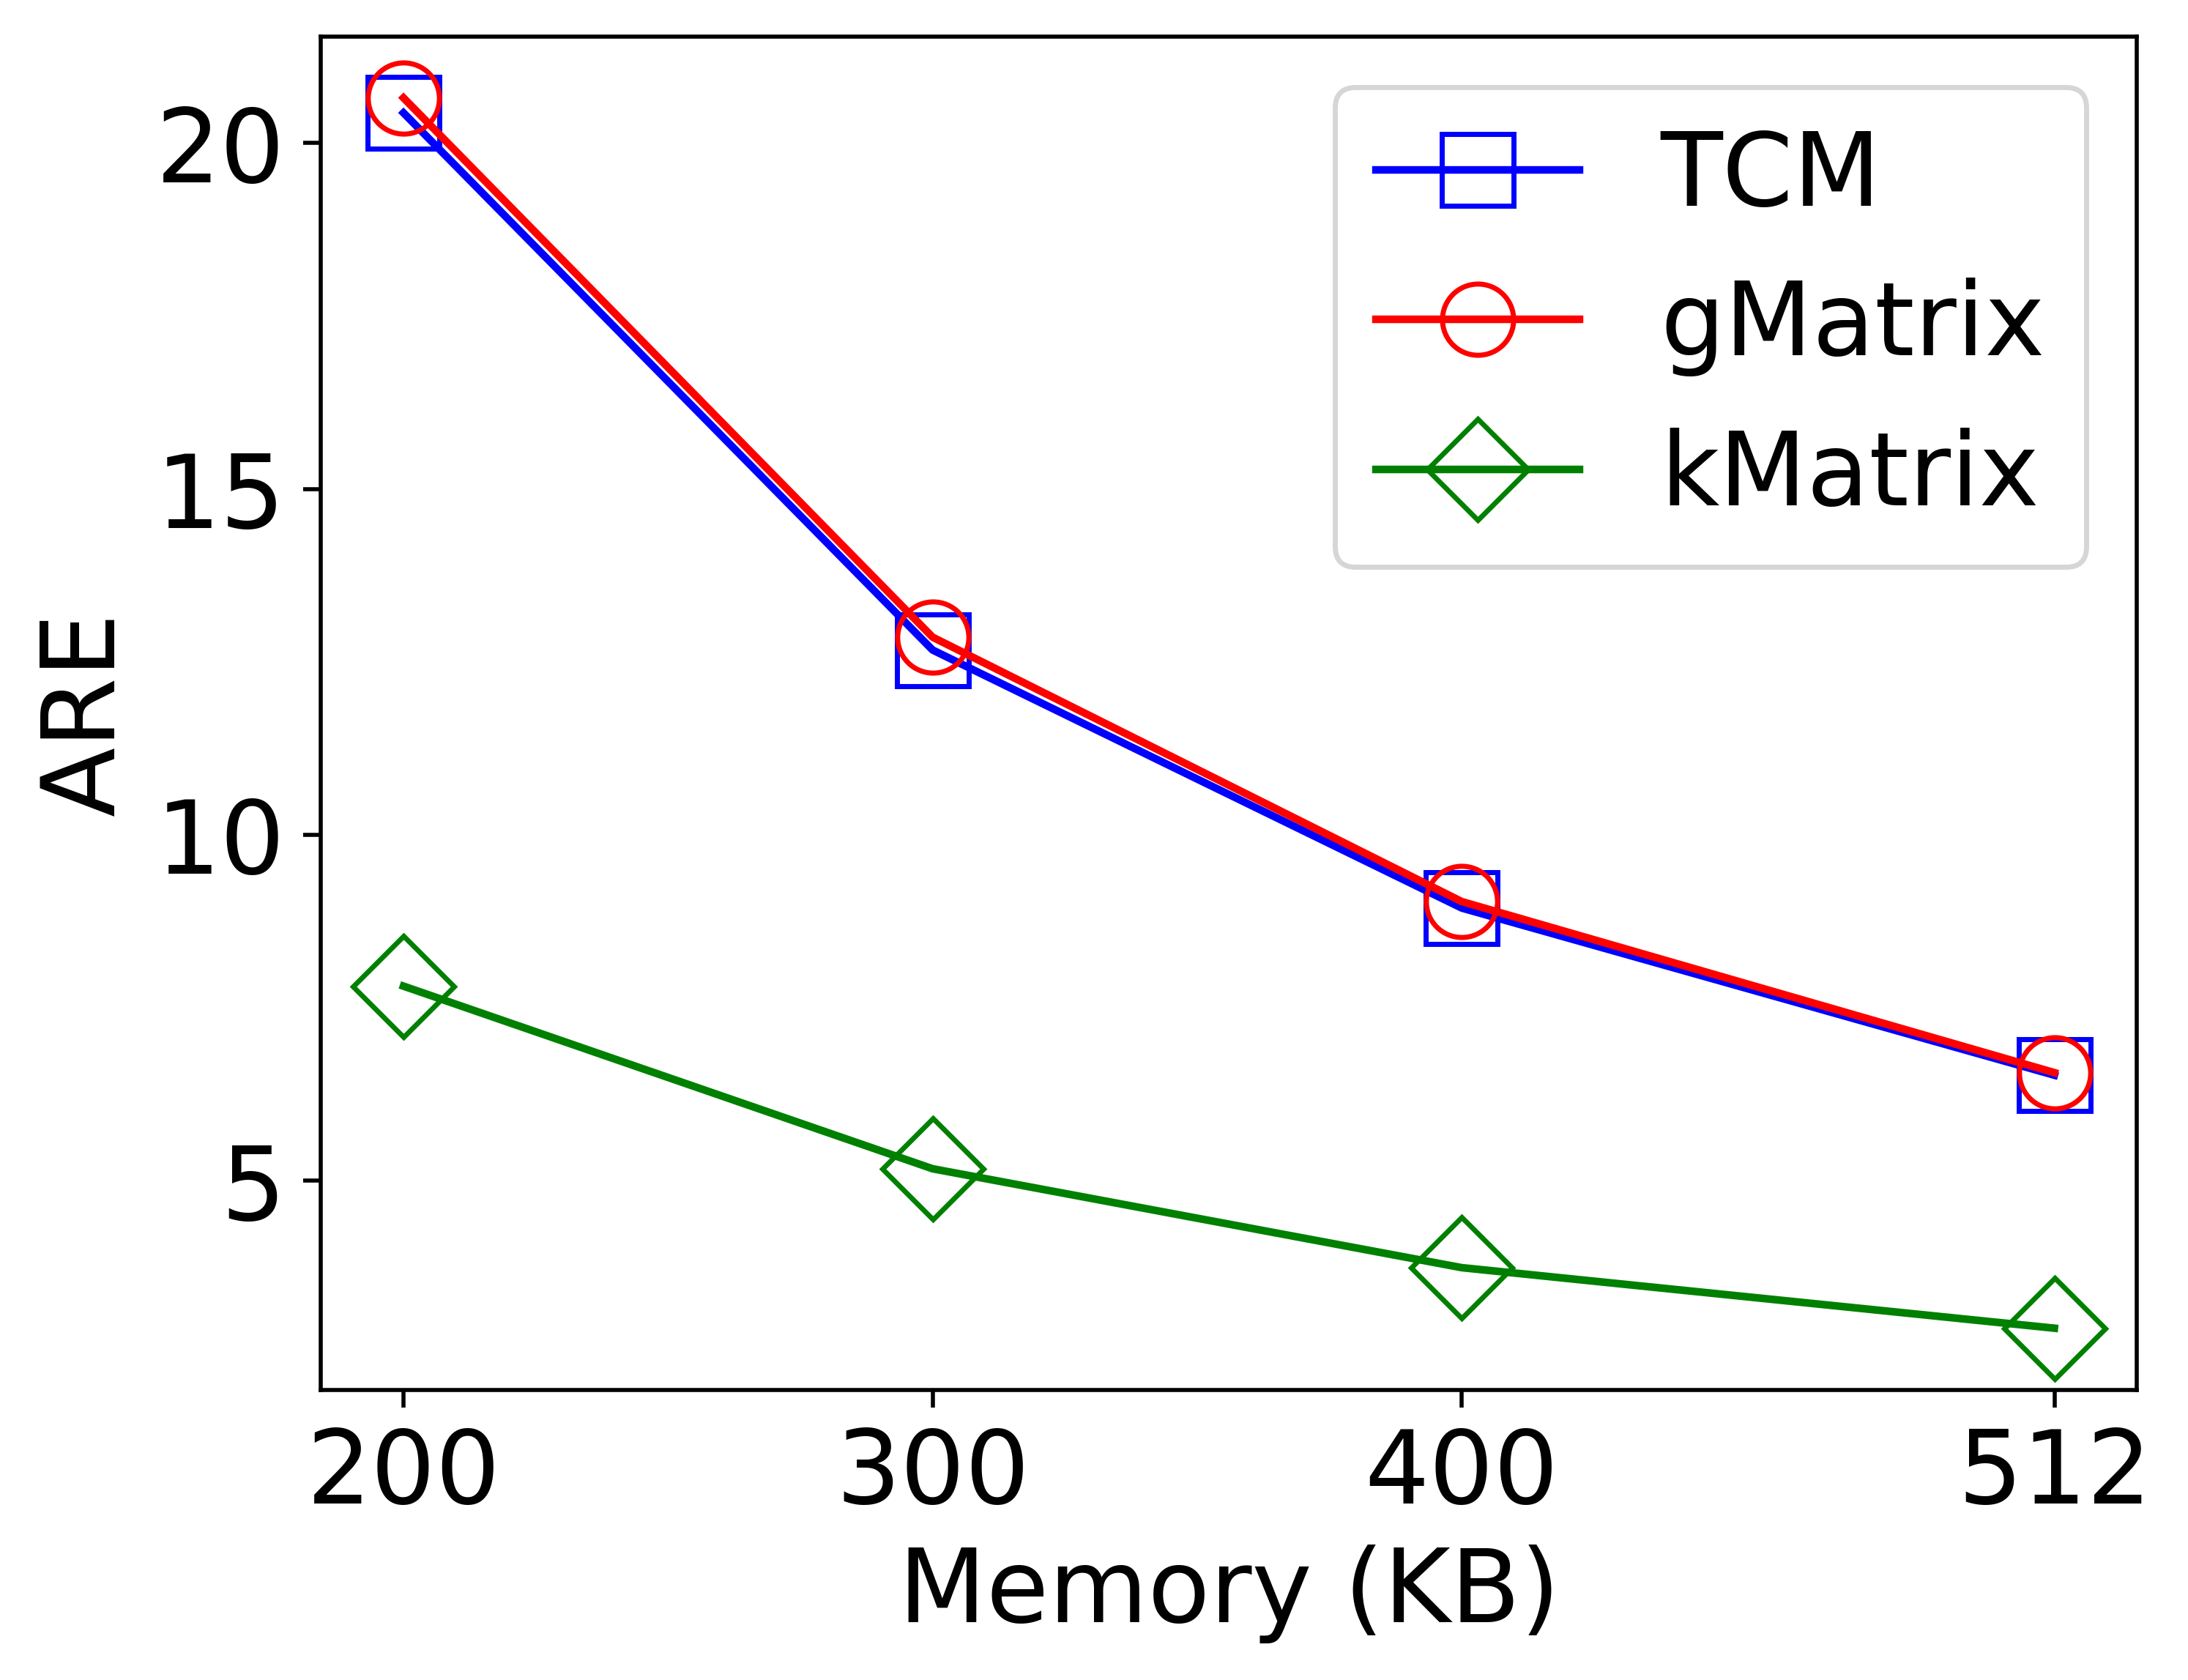
\includegraphics[width=0.45\linewidth]{img/edge_query_are_cit-HepPh.png}}
    \caption{Average relative error}
    \label{fig:edgq-queries-are-test}
\end{figure}

kMatrix showed significantly low ARE than all the other sketches for the three datasets we chose. The reason is that kMatrix can maintain frequency uniformity within each partition, making kMatrix relatively more immune to hash collisions than TCM and gMatrix. It is clear from the experimental evidence shown in Fig.~\ref{fig:edgq-queries-are-test} that kMatrix vastly outperforms the other state of the art sketching techniques. The superiority of our solution is more apparent when the allocated memory is low.

\subsubsection{Number of Effective Queries}

\begin{figure}[htbp] 
    \centering
    \subfloat[unicorn-wget\label{fig:neq-a}]{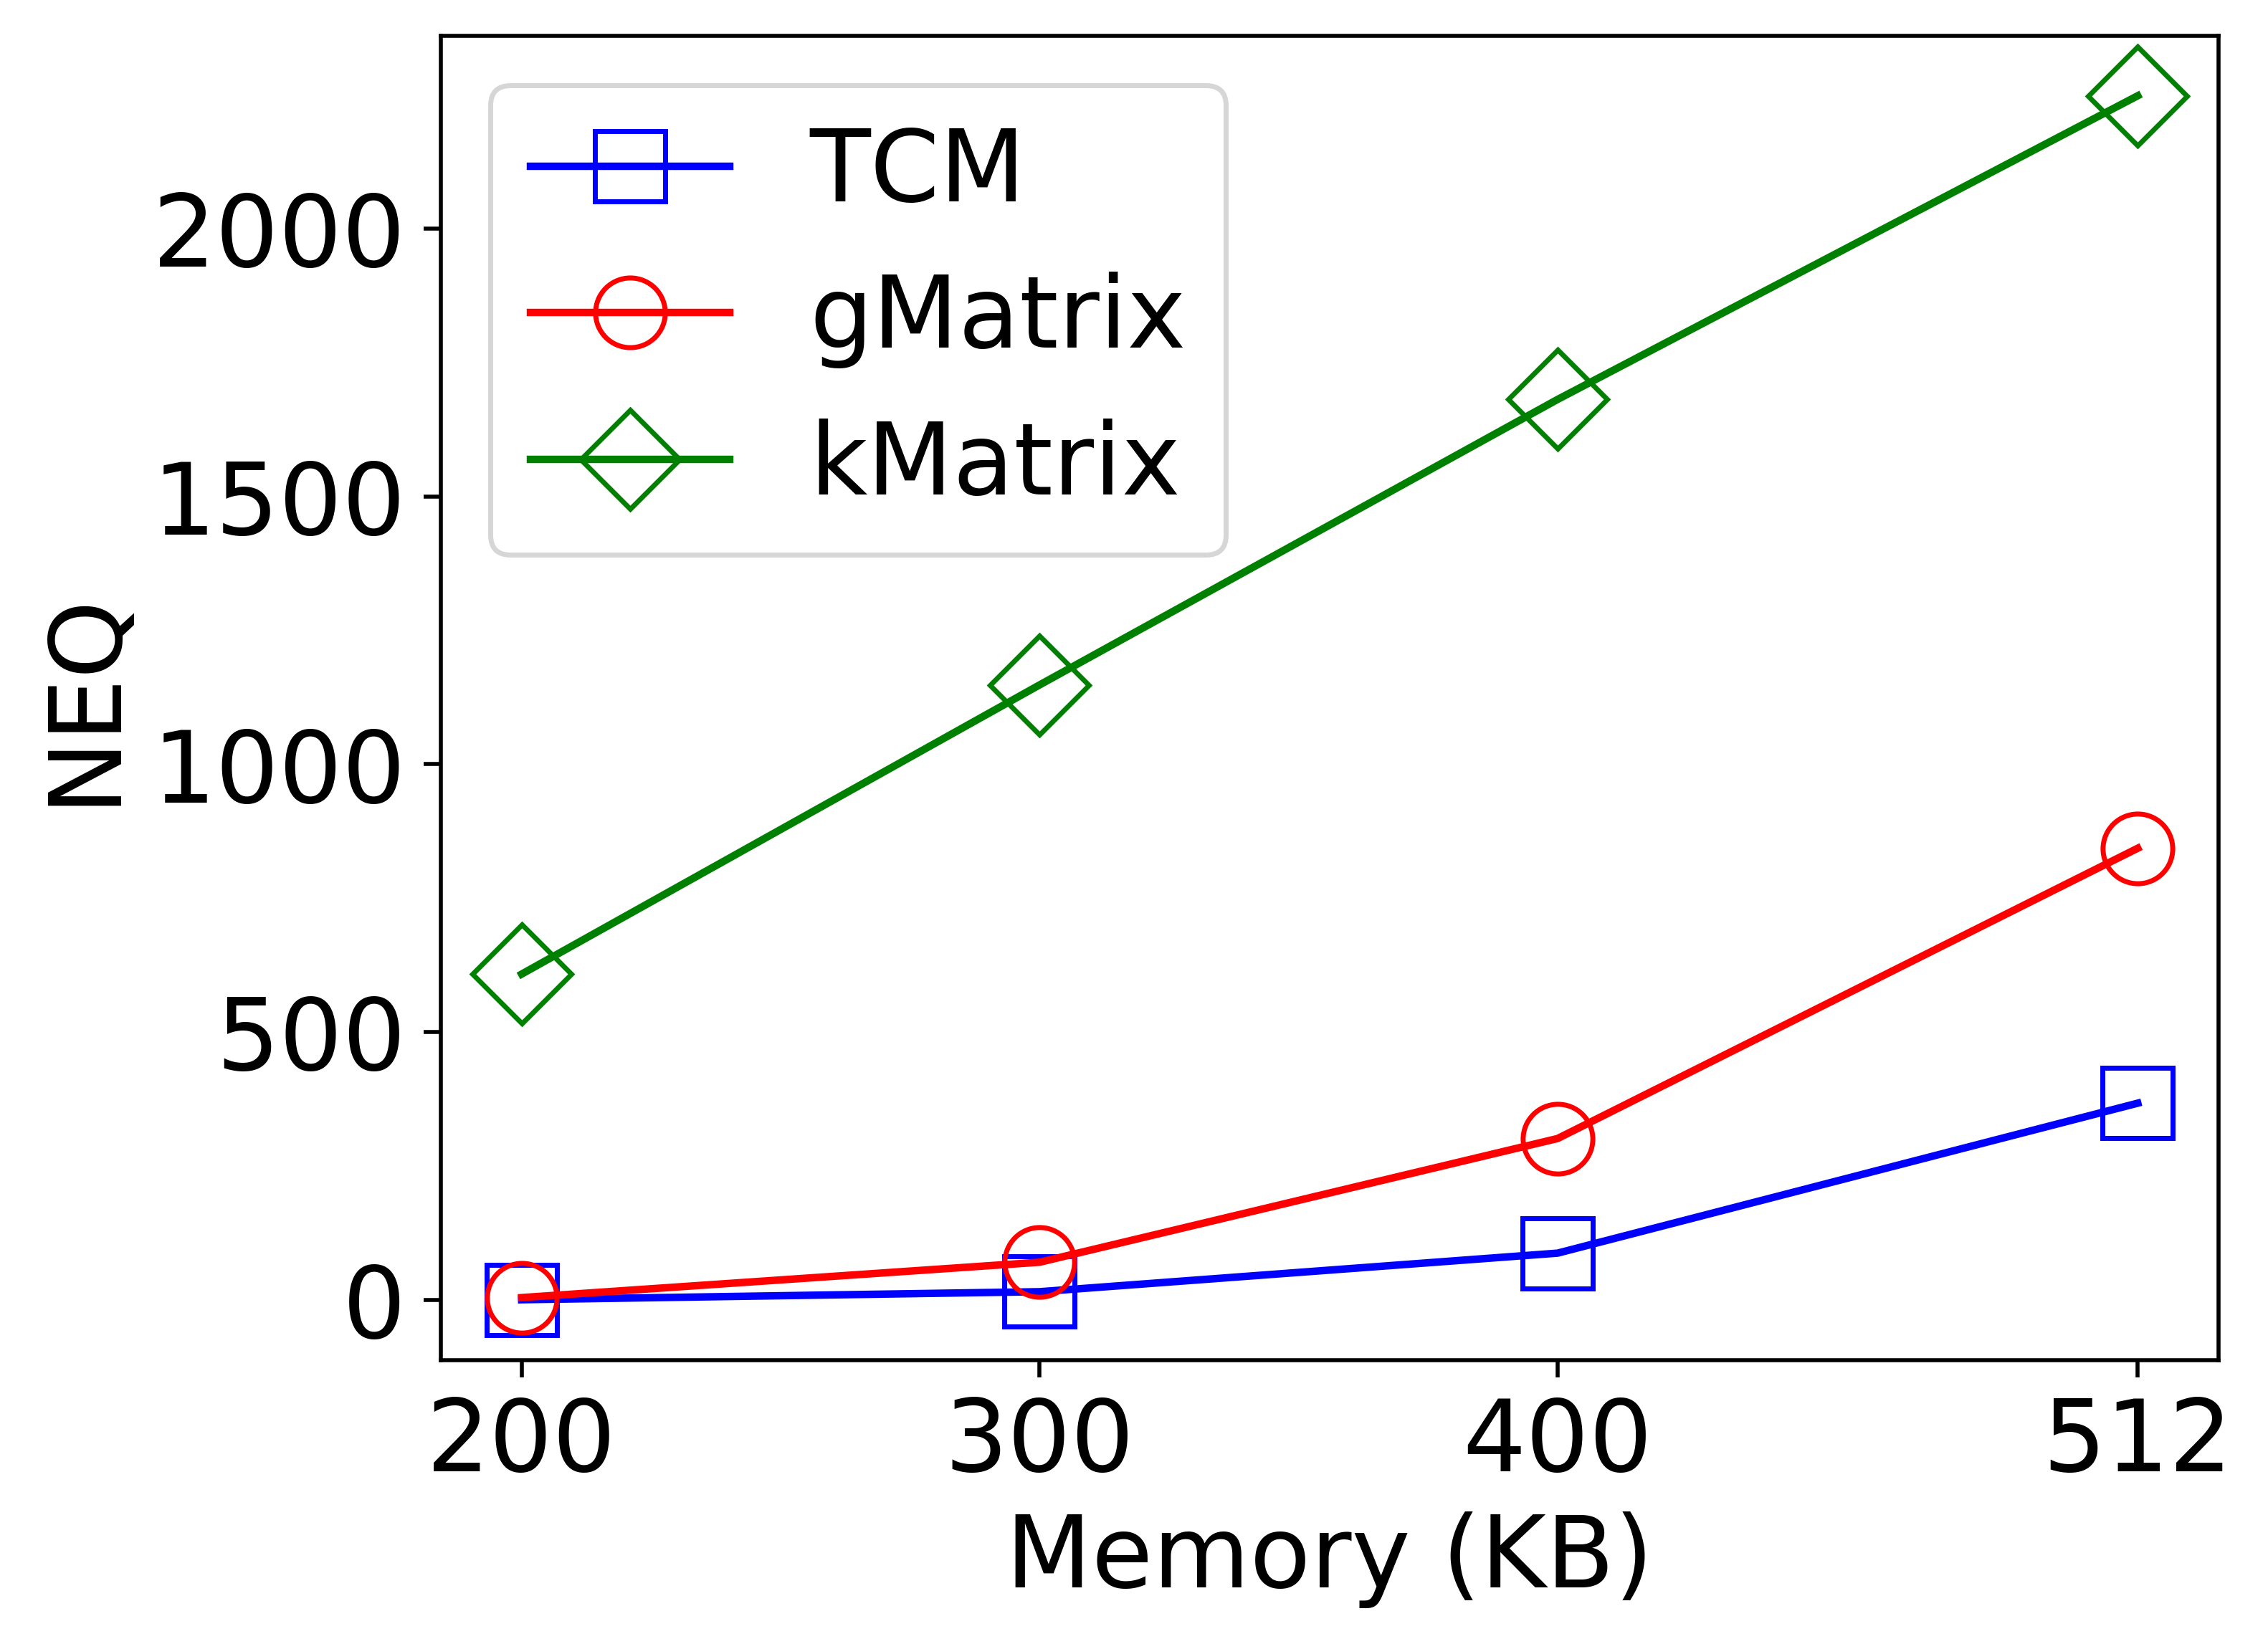
\includegraphics[width=0.45\linewidth]{img/edge_query_neq_unicorn-wget.png}}
    \hfill
    \subfloat[email-EuAll\label{fig:neq-b}]{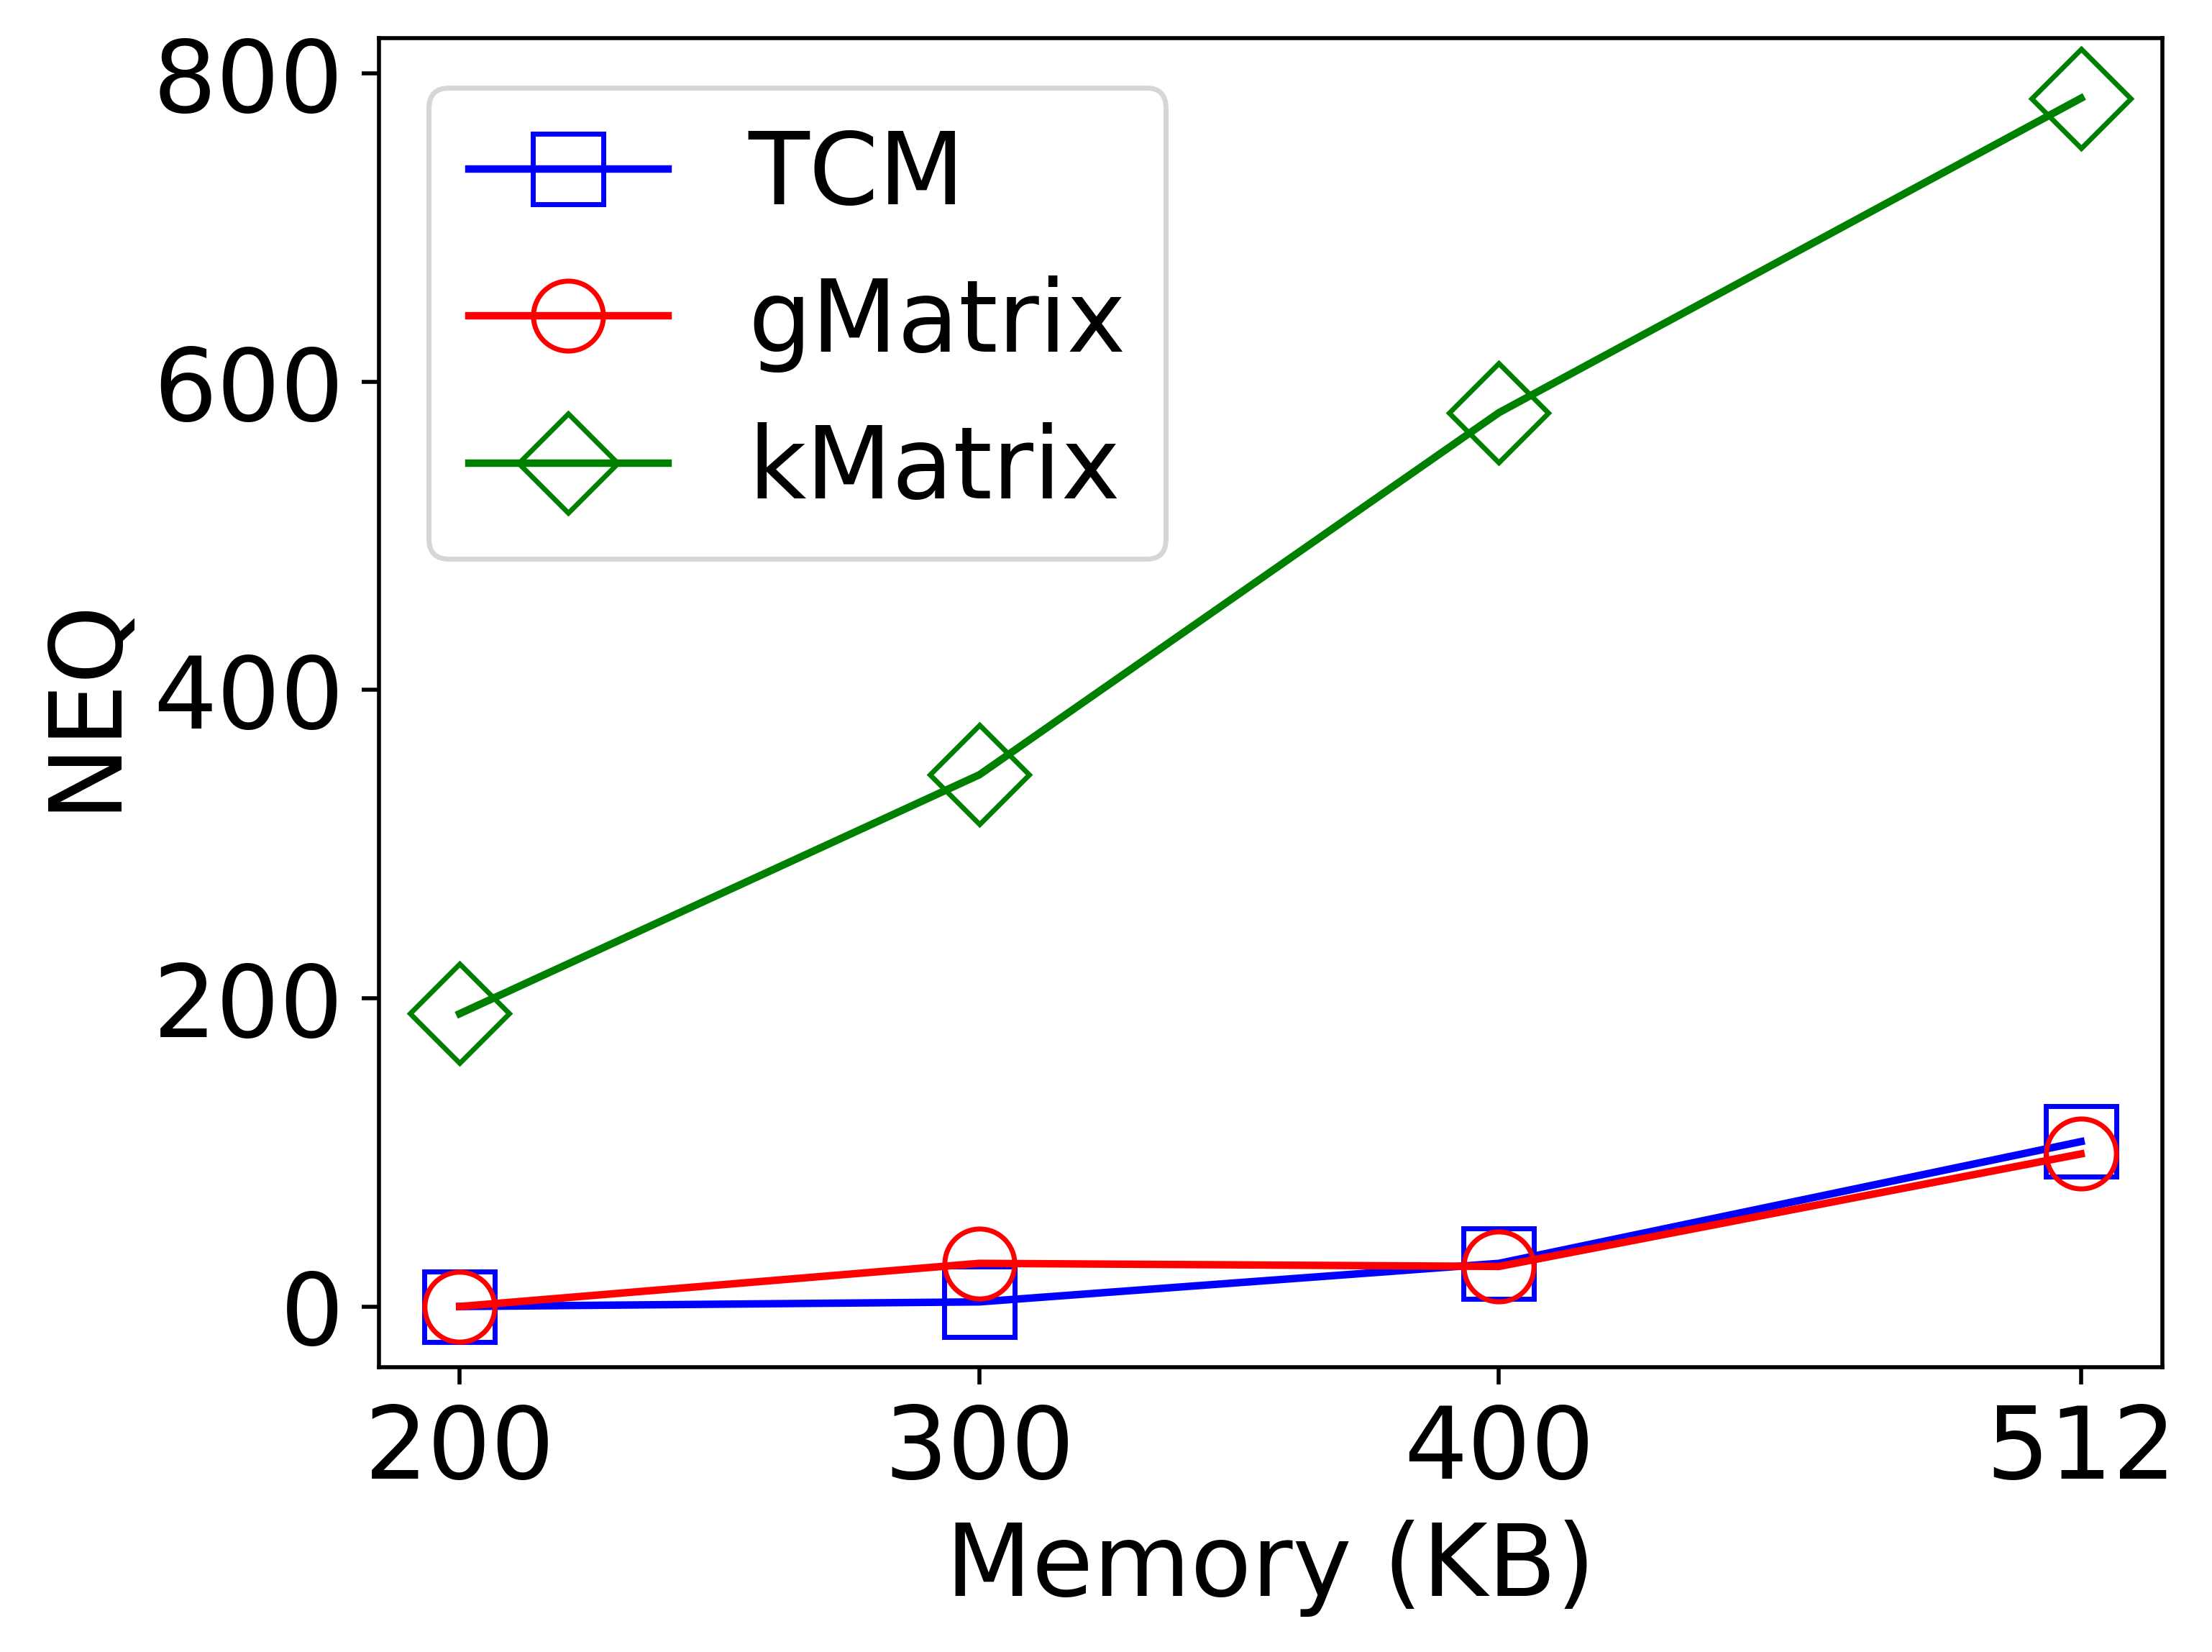
\includegraphics[width=0.45\linewidth]{img/edge_query_neq_email-EuAll.png}}
    \hfill
    \subfloat[cit-HepPh\label{fig:neq-c}]{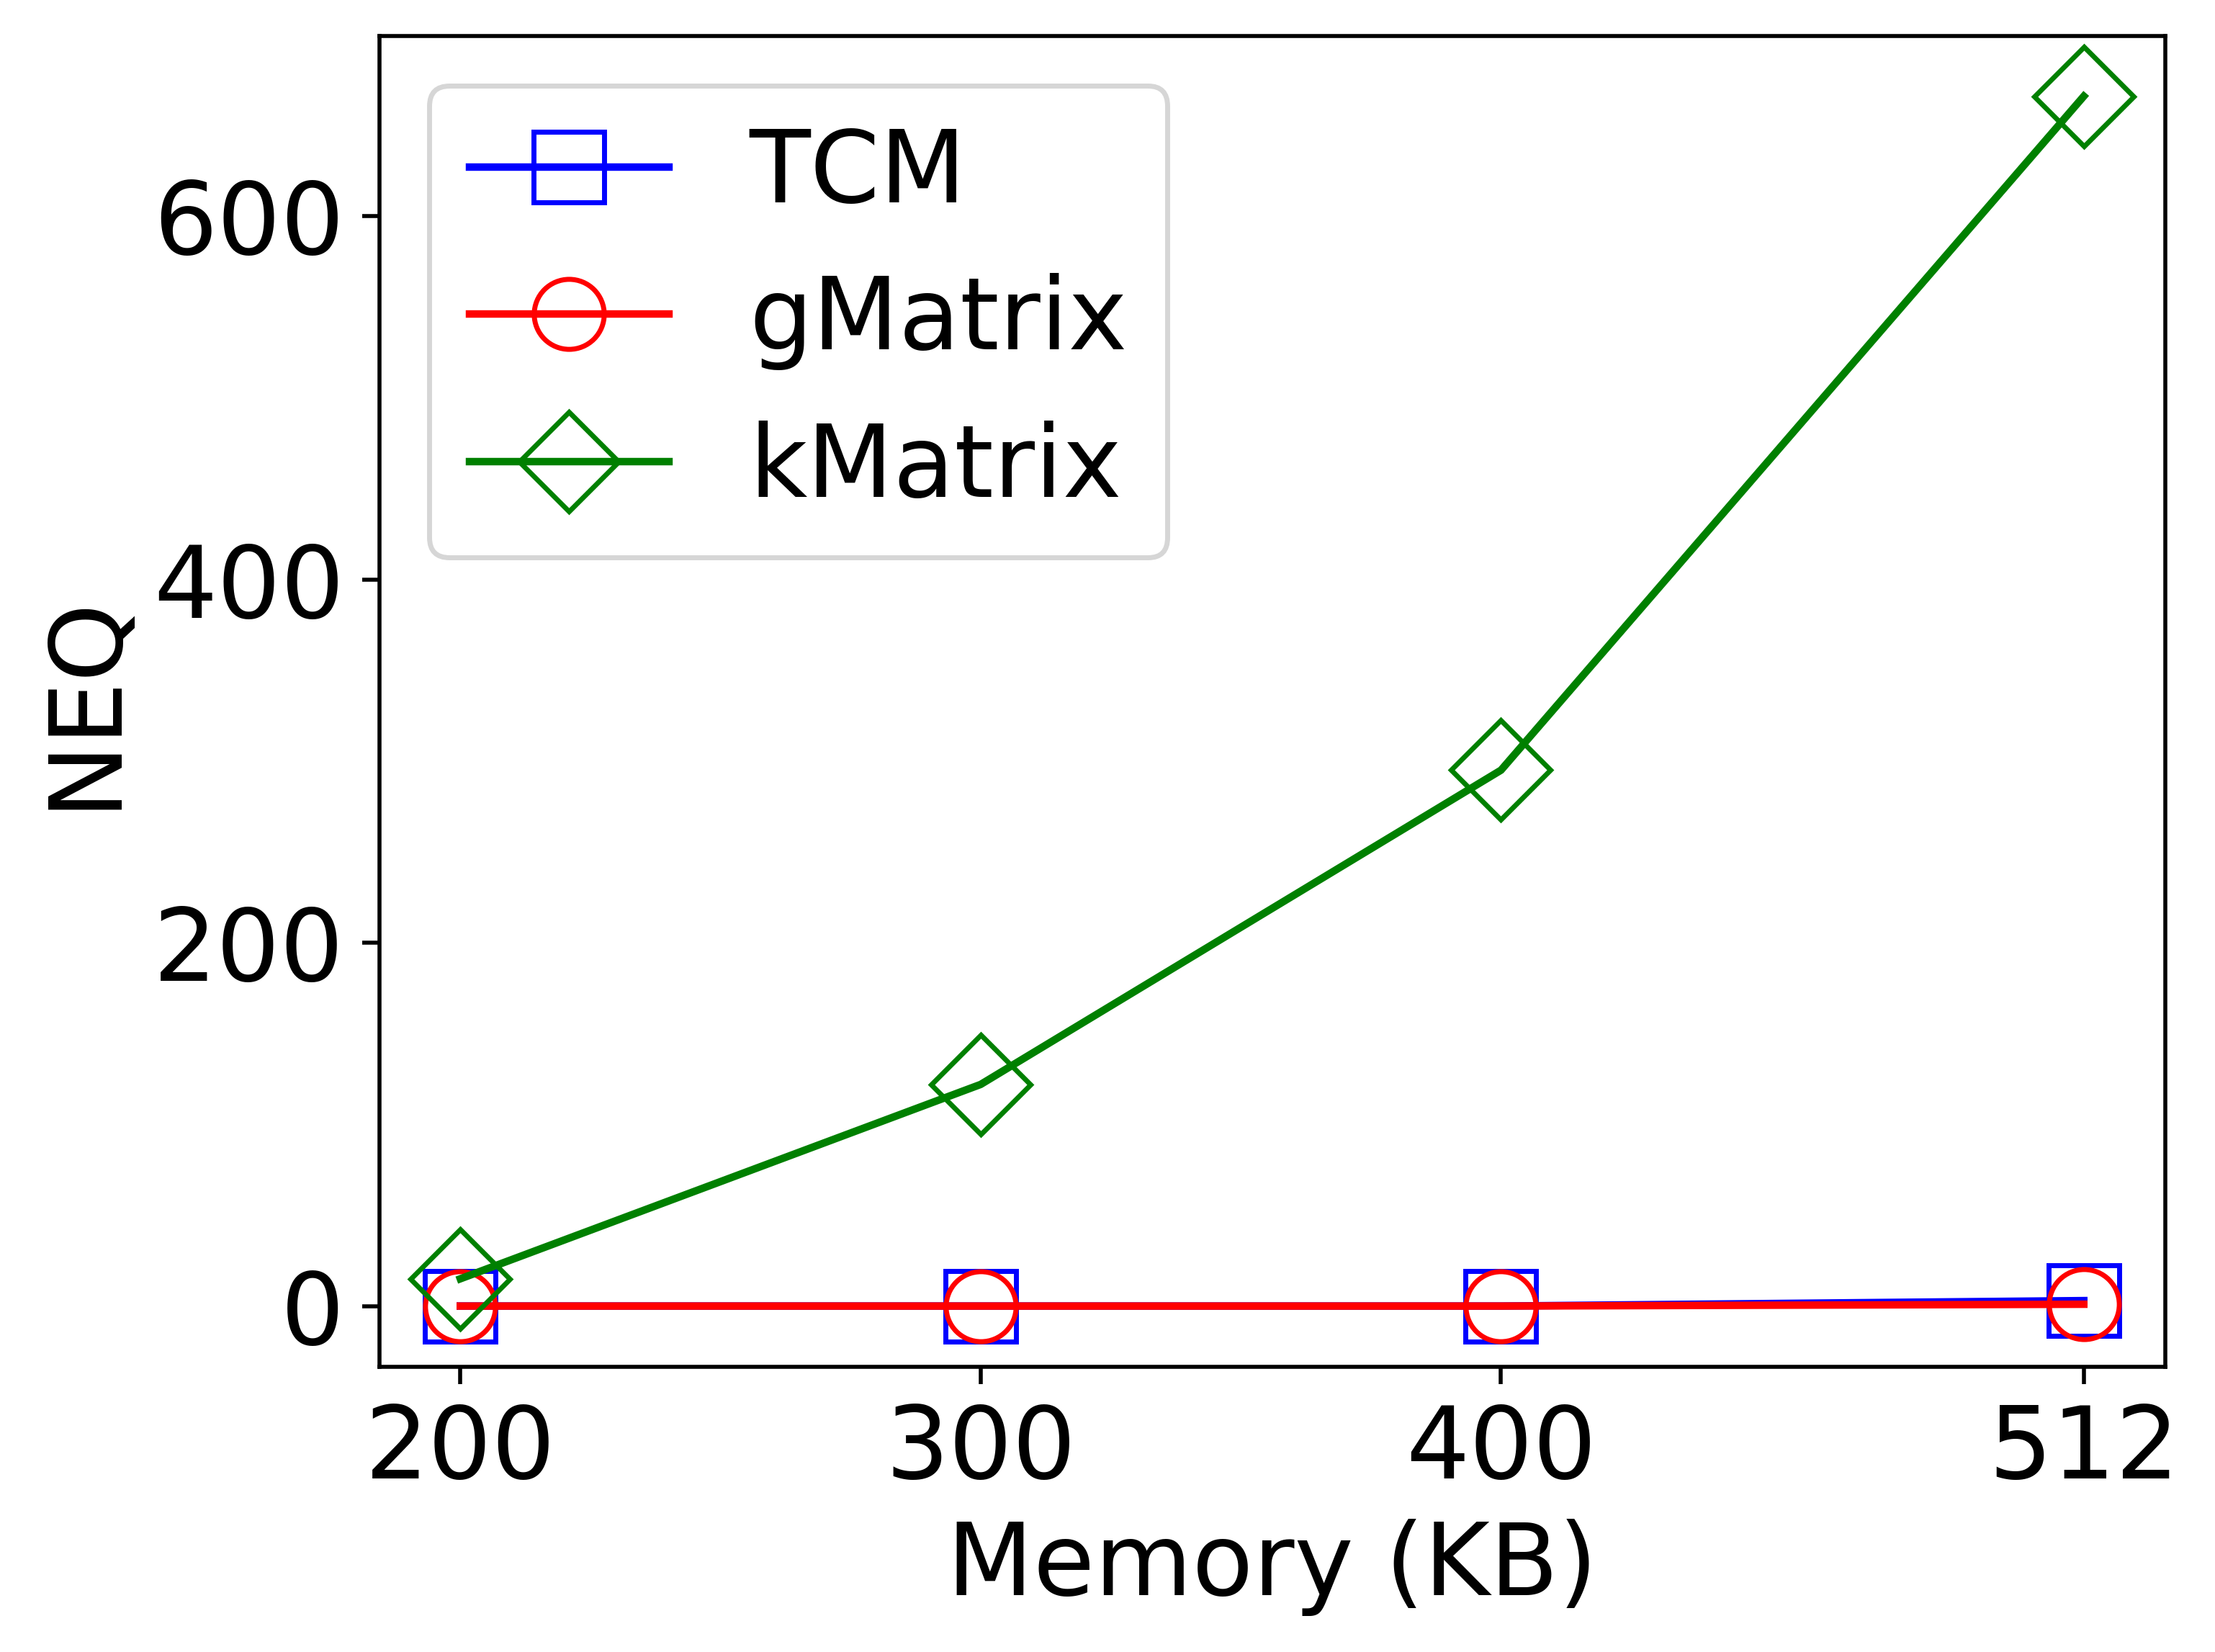
\includegraphics[width=0.45\linewidth]{img/edge_query_neq_cit-HepPh.png}}
    \caption{Number of effective queries}
    \label{fig:edgq-queries-neq-test}
\end{figure}

The number of effective queries for each sketch was calculated by querying the sketches against 10,000 edges chosen through reservoir sampling from the original dataset. kMatrix has surpassed the accuracy of both TCM and gMatrix for all the scenarios that we have tested. The results for cit-HepPh in Fig.~\ref{fig:neq-c} shows that kMatrix has been able to effectively answer a significantly larger number of queries where the other sketches failed due to hash collisions. This is due to the sketch partitioning process where kMatrix try to minimize the hash collisions in contrast to TCM and gMatrix.  
\section{Future work}

There are multiple aspects such as sliding windows and data partitioning across machines, that should be considered before the kMatrix sketch be used in a practical application. In addition, we have to test further the performance of kMatrix concerning other criteria such as heavy node/edge queries. The test suit’s functionalities can be extended and improved upon as a benchmarking tool for testing the graph summarization sketches. 
\section{Conclusion}

kMatrix is a new streaming graph summarization technique proposed through this research. It can answer queries with a significantly lower average relative error with the same amount of memory compared to the existing state-of-the-art sketching techniques, TCM and gMatrix. We have benchmarked kMatrix using three datasets in different application domains. We believe that the experimental results show the superiority of the proposed solution in comparison to the existing steaming graph summarization techniques. 

\bibliographystyle{ieeetr}
\bibliography{ms}

\end{document}
